% !TeX spellcheck = en_GB

%	PACKAGES AND OTHER DOCUMENT CONFIGURATIONS
%----------------------------------------------------------------------------------------

\documentclass[twoside]{article}



\usepackage[sc]{mathpazo} % Use the Palatino font
\usepackage[T1]{fontenc} % Use 8-bit encoding that has 256 glyphs
\linespread{1.05} % Line spacing - Palatino needs more space between lines
\usepackage{microtype} % Slightly tweak font spacing for aesthetics

\usepackage[hmarginratio=1:1,top=32mm,columnsep=20pt]{geometry} % Document margins
\usepackage{multicol} % Used for the two-column layout of the document
\usepackage[hang, small,labelfont=bf,up,textfont=it,up]{caption} % Custom captions under/above floats in tables or figures
\usepackage{booktabs} % Horizontal rules in tables
\usepackage{float} % Required for tables and figures in the multi-column environment - they need to be placed in specific locations with the [H] (e.g. \begin{table}[H])
\usepackage{hyperref} % For hyperlinks in the PDF


% % % % My packages

\usepackage{psfrag}
\usepackage[center]{subfigure}
\usepackage{subfloat}
\usepackage{float}
\usepackage{longtable}
\usepackage{amsmath} 
\usepackage{amsfonts} % Permet l'utilisation de plus de polices de caractères en mode mathématique
\usepackage[dvips]{graphicx} % Pour utiliser la commande \includegraphics
\usepackage{slashbox}
\usepackage{graphicx}
\usepackage{transparent}
\usepackage{multirow}
\usepackage{color}
\usepackage[svgnames]{xcolor}
\usepackage{xparse}	% used to define new commands


% % % % % % % % % % % % % % % % % % % %


%% Format de la page
%\setlength{\marginparsep}{0.0cm}%
%\setlength{\marginparwidth}{0.0cm}%
%\setlength{\oddsidemargin}{0.0cm}%
%\setlength{\evensidemargin}{0.0cm}%
%\setlength{\textwidth}{16cm}%
%\setlength{\topmargin}{0.0cm}%
%\setlength{\textheight}{20cm}%




% % % % % % % % % % % % % % % % % % % % % %
\usepackage{lettrine} % The lettrine is the first enlarged letter at the beginning of the text
\usepackage{paralist} % Used for the compactitem environment which makes bullet points with less space between them

\usepackage{abstract} % Allows abstract customization
\renewcommand{\abstractnamefont}{\normalfont\bfseries} % Set the "Abstract" text to bold
\renewcommand{\abstracttextfont}{\normalfont\small\itshape} % Set the abstract itself to small italic text

\usepackage{titlesec} % Allows customization of titles
\renewcommand\thesection{\Roman{section}} % Roman numerals for the sections
\renewcommand\thesubsection{\Roman{subsection}} % Roman numerals for subsections
\titleformat{\section}[block]{\large\scshape\centering}{\thesection.}{1em}{} % Change the look of the section titles
\titleformat{\subsection}[block]{\large}{\thesubsection.}{1em}{} % Change the look of the section titles

\renewcommand{\baselinestretch}{3} % Changer l'interligne

% New commands
\DeclareDocumentCommand \N { m } {	% 1 mandatory arg (shape)
	N^{#1}
}

 % Pour la numérotation différente des sous sections
 \setcounter{secnumdepth}{3}
 
 \renewcommand   \thesection         {\Roman{section}}
 \renewcommand   \thesubsection      {\thesection.\arabic{subsection}}
 \renewcommand   \thesubsubsection       {\alph{subsubsection}}


% %Mes macros
\newcommand\point{\stackrel{.}}
\newcommand\tw{tw} % notation de largeur de trabsition
\newcommand\noise{\mathcal{N}} %Notation bruit
\newcommand\Smo{\bar} %Notation de l'image lissée
\newcommand\D{I^{CFAD}} %Notation des dirivées partielles de Deriche de l'image CFA
\newcommand\Dplus{I^{CFAD^+}}
\newcommand\Dmoins{I^{CFAD^-}}




\DeclareMathOperator{\e}{e}
%-----------------------------------------------------------------------------------
%	TITLE SECTION
%-----------------------------------------------------------------------------------

\title{\vspace{-15mm}\fontsize{24pt}{10pt}\selectfont\textbf{Edge detection from Bayer CFA images}} % Article title

\author{
\large
\textsc{Arezki ABERKANE$^{1}$, Olivier LOSSON$^{2}$ and Ludovic MACAIRE$^{3}$}\\[2mm] % Your name
\normalsize Laboratoire CRIStAL, Universit\'e Lille1 - Sciences et Technologies,\\ \normalsize Cit\'e scientifique - B\^atiment P2, 59650 Villeneuve d'Ascq Cedex, France \\ % Your institution
\normalsize \href{mailto:arezki.aberkane@ed.univ-lille1.fr}{$^{1}$arezki.aberkane@ed.univ-lille1.fr},  
\href{mailto:olivier.losson@univ-lille1.fr}{$^{2}$olivier.losson@univ-lille1.fr},  
\href{mailto:ludovic.macaire@univ-lille1.fr}{$^{3}$ludovic.macaire@univ-lille1.fr} % Your email address
\vspace{-5mm}
}
\date{}

%----------------------------------------------------------------------------------------

\begin{document}

\maketitle % Insert title

%\thispagestyle{fancy} % All pages have headers and footers

%----------------------------------------------------------------------------------------
%	ABSTRACT
%----------------------------------------------------------------------------------------

\begin{abstract}
  

\end{abstract}

%----------------------------------------------------------------------------------------
%	ARTICLE CONTENTS
%----------------------------------------------------------------------------------------

% %\begin{multicols}{2} % Two-column layout throughout the main article text

\section{Introduction}

There are two major families of digital colour cameras: cameras with three sensors where each captures one of the three primary colours (red, green, or blue) and those with a single sensor. Although the digital cameras with three sensors are very effective and give  excellent images,  this technology is very onerous and cumbersome, which is prohibitive for most consumers. For these reasons, most digital colour cameras nowadays embed only a single sensor. Such cameras are fitted with a Colour Filter Array (CFA) and deliver CFA images, in which each pixel is characterized by only one out of the three colour components (red, green, or blue), and that must be interpolated to estimate the full colour images. This process is known as demosaicing (or demosaicking).

Most demosaicing schemes are dedicated to the widespread Bayer CFA that is presented in section~\ref{sec:CFA_demosaicing} together with the demosaicing problem. Review papers about the many demosaicing schemes proposed in the literature were conducted by Gunturk et al.~\cite{gunturk_ip_2002,li_vcip_2008} and most recently by Menon and Calvagno~\cite{menon_ic_2011}. Since demosaicing is not our main concern and we precisely aim at avoiding it, we only give a quick insight of the main strategies that have been used to this aim. We especially focus on the most recent and efficient state-of-the-art algorithms, as well as on issues related to CFA image noise.

% Many more sophisticated methods are available in the literature. They are based on constant-hue~\cite{cok_icps_1994} and/or gradient-based interpolation~\cite{hibbard_patent_1995,hamilton_patent_1997} that rely on an edge preservation strategy or approaches based on spectral correlation \cite{alleysson_ip_2005}. Chung et al.~\cite{chung_ip_2008} combine the gradient/edge information extracted from the CFA image and the adaptive heterogeneity-projection value into a new edge-sensing demosaicing algorithm. Currently, the best demosaicing algorithms in terms of PSNR are proposed by Pekkucuksen and Altunbasak~\cite{pekkucuksen_ip_2013} and by Kiku et al.~\cite{kiku_icip_2013}. These are hybrid demosaicing algorithms because they are based on the spatial and spectral correlations.

Demosaicing methods are generally designed to produce ``perceptually satisfying'' images, but do not consider how resultant artefacts would affect a subsequent analysis of these images. In a previous work~\cite{losson_aiep_2010} we show that demosaicing is detrimental to low-level image analysis because it often fails to reconstruct the high-frequency information correctly. Focusing on the various demosaicing artefacts, we propose specific measurements to quantify how each of them specifically occurs and affects edge detection in the demosaiced image. Other studies confirm the latter and show that demosaicing alters the texture representation quality in particular, and that the CFA image can be used effectively for colour texture classification~\cite{losson_ietip_2012, losson_cviu_2013}. However, very few works similarly try to use the CFA image directly for low-level image analysis. Chen et al.~\cite{chen_apccas_2006} investigate the feasibility of edge detection by a dedicated Gaussian smoothing and Laplacian-based edge kernels which can be applied to a CFA image. Despite that this method is visually highly noise-sensitive and has not been objectively evaluated, its encouraging results lead us to investigate edge detection from CFA images to avoid artefacts generated by the demosaicing process. 

To perform edge detection directly on the CFA image, we adapt Di Zenzo's vector gradient~\cite{zenzo_cvgip_1986} to the CFA image. The colour gradient is based on a tensor of the first derivatives of colour component images. Our main contribution is to adapt these derivative estimation to the CFA image where two colour component levels are missing at each pixel, as presented in section \ref{sec:gradients}.

%The rest of this paper is organized as follows. We first present the considered CFA image, the demosaicing problem and state-of-the-art algorithms, including  issues related to CFA image noise. In section \ref{sec:gradients}, we propose a new approach of edge detection from the CFA image. Then, some experiments are carried out to assess the performance and robustness of the proposed method. Finally, some conclusions are addressed in the last section.


%-----------------------------------------------------------------------
\section{CFA demosaicing}
\label{sec:CFA_demosaicing}
%-----------------------------------------------------------------------

%-----------------------------------------------------------------------
\subsection{Demosaicing problem formulation}
\label{subsec:problem_formulation}

Most of single-sensor cameras are fitted with a Bayer CFA, which is exclusively considered in this paper. Such cameras provide a raw image denoted as $I^{CFA}$ and shown in Fig.~\ref{fig:Bayer CFA image}. The set $S$ of all image pixels can be divided into $S = S^R \cup S^G \cup S^B$, where $S^k$ denotes the set of pixels where the colour component $k$ is available in $I^{CFA}$ (see Figs.~\ref{fig:S^R}--\ref{fig:S^G}). Both $S^R$ and $S^B$ contain pixels arranged in a regular lattice (a quarter of all pixels), and $S^G$ contains (half of all) pixels arranged in a quincunx lattice. It can be further divided into $S^G = S^{G,R} \cup S^{G,B}$, where $S^{G,k}$ ($k \in \{R,B\}$) is the subset of $S^G$ pixels whose horizontal neighbours belong to $S^k$ (see Figs.~\ref{fig:S^G,R} and \ref{fig:S^G,B}).


\begin{figure}[H]
	\centering
	\subfigure[$I^{CFA}$]{
		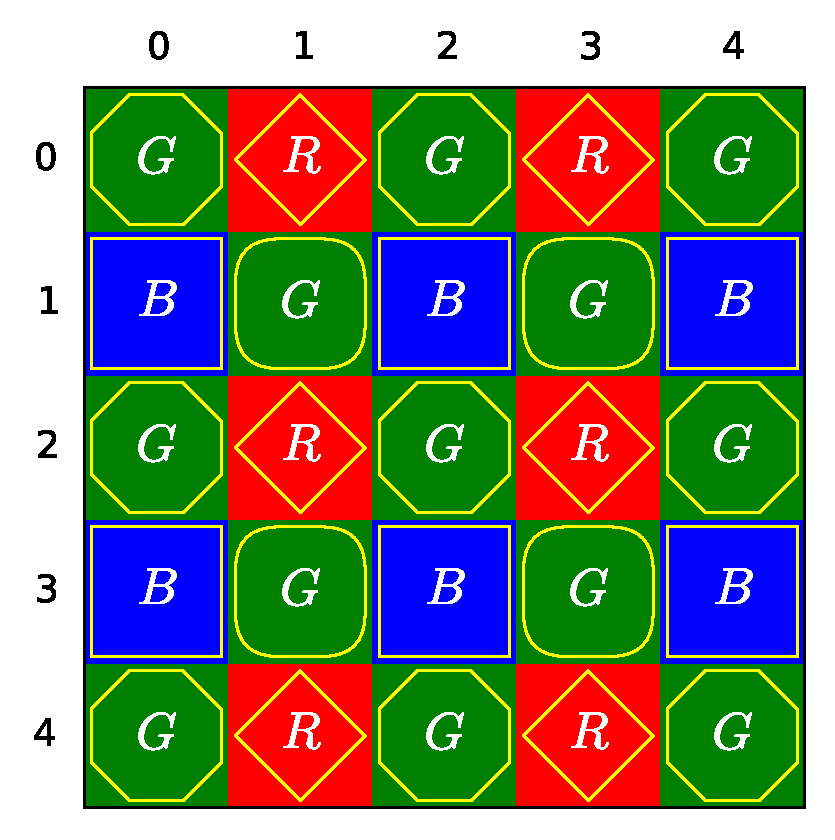
\includegraphics[width=0.27\linewidth]{fig/I^CFA} 
		\label{fig:Bayer CFA image}
	}
	\quad
	\subfigure[$S^R$]{
		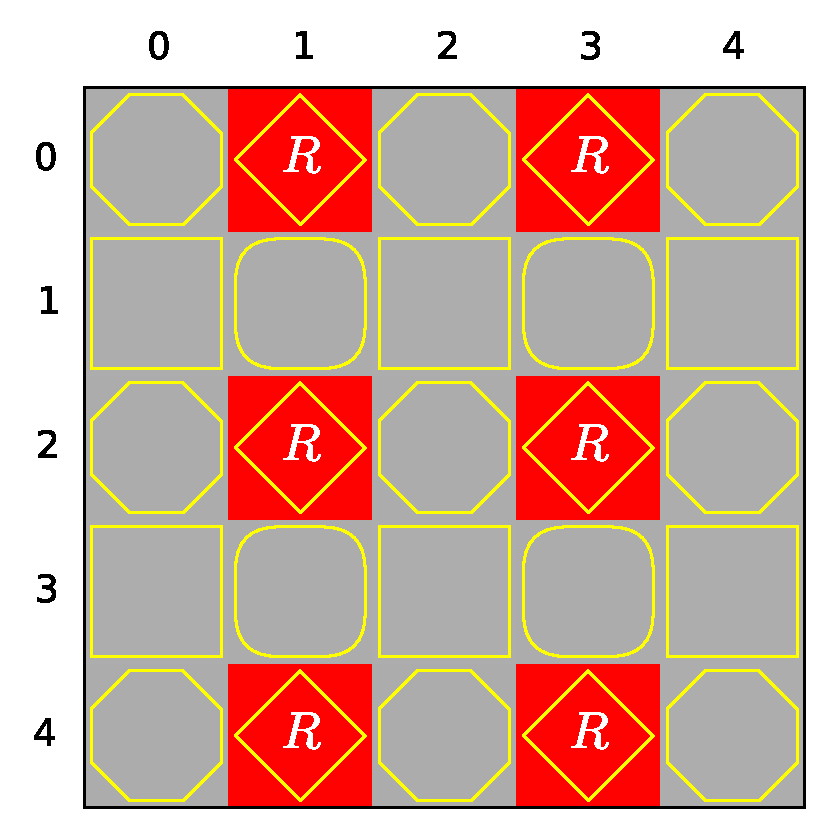
\includegraphics[width=0.27\linewidth]{fig/S^R} 
		\label{fig:S^R}	 
	}
	\quad
	\subfigure[$S^B$]{
		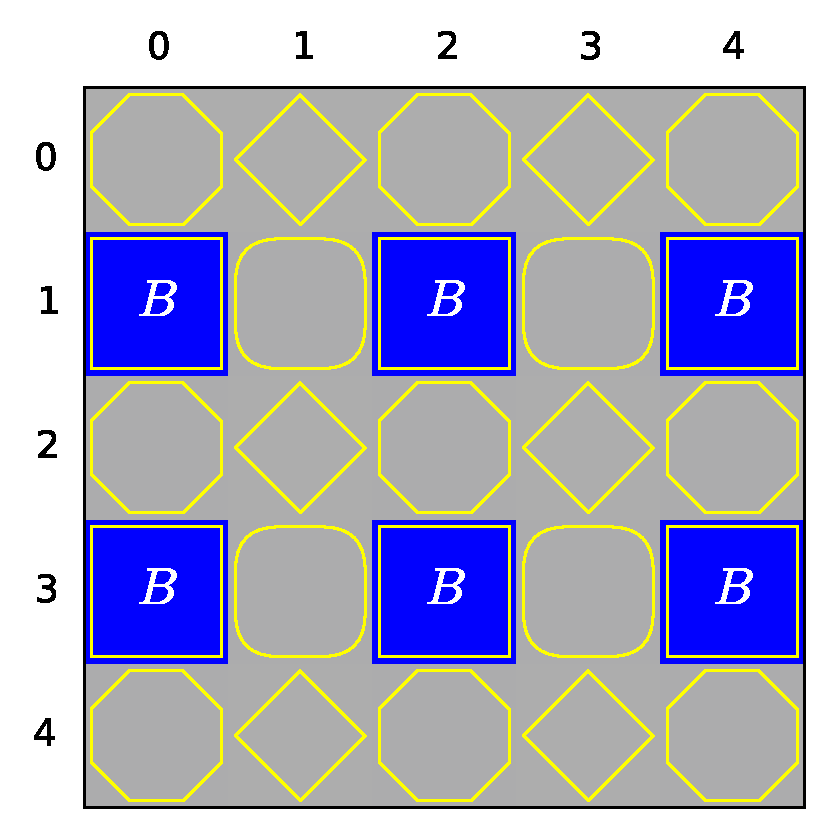
\includegraphics[width=0.27\linewidth]{fig/S^B} 
		\label{fig:S^B}
	}
	\\
	\subfigure[$S^G$]{
		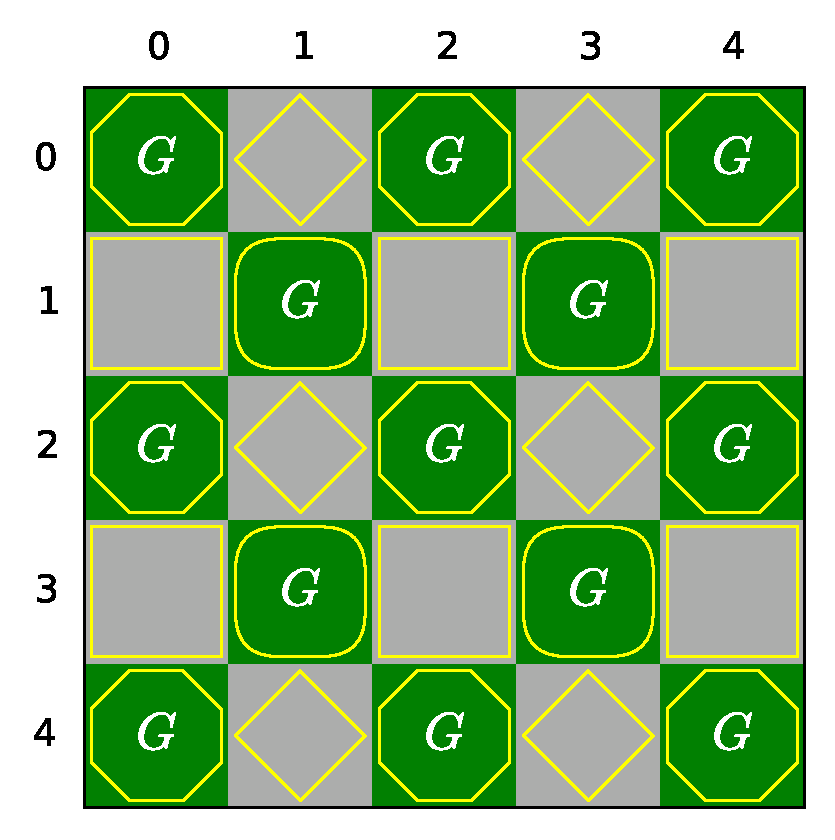
\includegraphics[width=0.27\linewidth]{fig/S^G} 
		\label{fig:S^G}	 
	}
	\quad
	\subfigure[$S^{G,R}$]{
		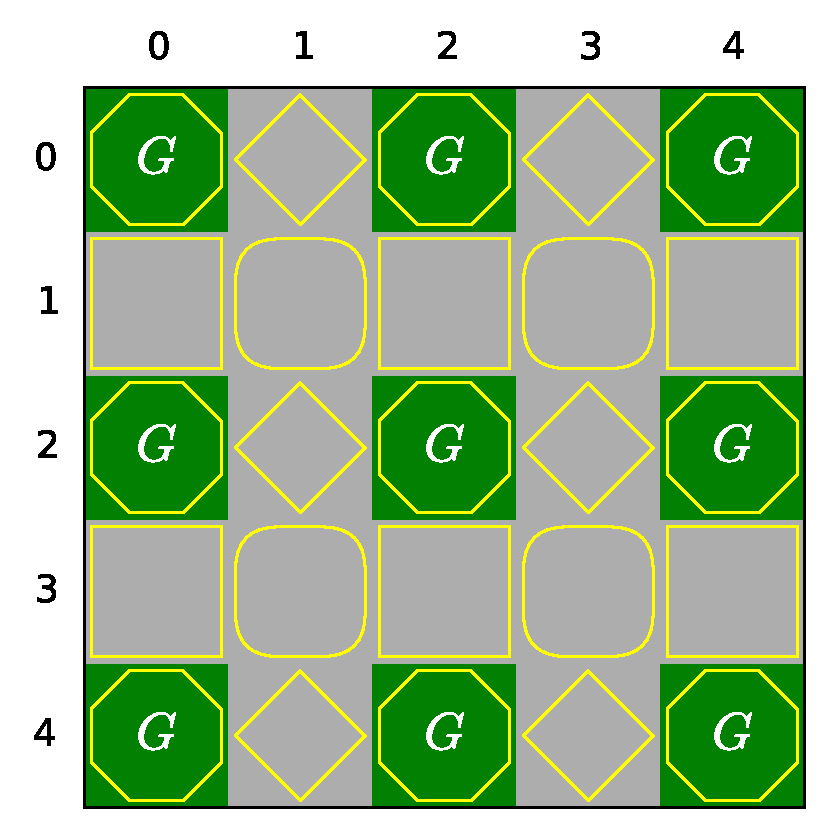
\includegraphics[width=0.27\linewidth]{fig/S^G,R}
		\label{fig:S^G,R} 
	}
	\quad
	\subfigure[$S^{G,B}$]{
		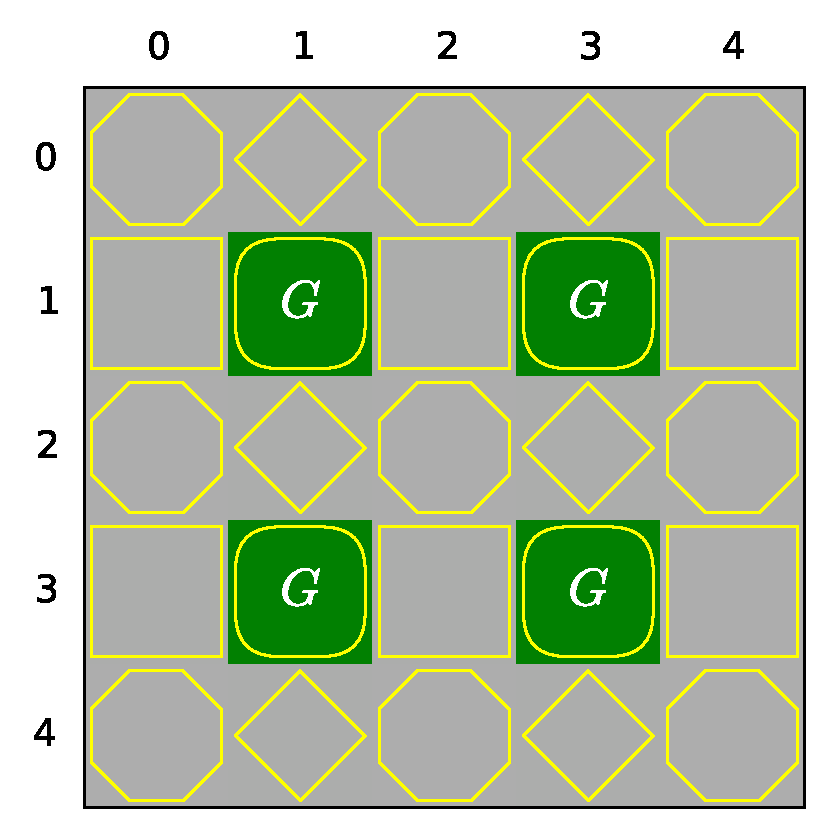
\includegraphics[width=0.27\linewidth]{fig/S^G,B}
		\label{fig:S^G,B}
	}

	\caption[Bayer CFA image and component-wise pixel subsets.]{Bayer CFA image and component-wise pixel subsets. The notations $R$, $G$, and $B$ express that the level of the respective colour component is available at that location.}
	\label{fig: Bayer CFA and the component image}
\end{figure}



%We consider $P$, the pixel in $I^{CFA}$ with spatial coordinates $(x,y)$, the single colour component available at $P(x,y)$ in $I_{CFA}$ is:  
%
%\begin{eqnarray}I^{CFA}(P) =
%	\left\lbrace
%	\begin{array}{ccc}
%		I^R(P) & & \text{if $P \in S^R$,}  \\
%		I^G(P) & & \text{if $P \in S^G$,}\\
%		I^B(P) & & \text{if $P \in S^B$,}
%	\end{array}\right.
%	\label{eq:I--ICFA}	
%\end{eqnarray}


To determine the colour of each pixel $P$ in the estimated colour image $\hat{\textbf{I}}$, the demosaicing process generally retains the colour component available at the same location in $I^{CFA}$, and estimates the missing other two components:

\begin{eqnarray}\hat{\textbf{I}}(P) =
	\left\lbrace
	\begin{array}{ccc}
		\left(I^{CFA}(P),\hat{I}^G(P), \hat{I}^B(P) \right)^T & & \text{if $P \in S^R$,}\\
		\left(\hat{I}^R(P),I^{CFA}(P), \hat{I}^B(P) \right)^T & & \text{if $P \in S^G$,}\\
		\left(\hat{I}^R(P),\hat{I}^G(P), I^{CFA}(P) \right)^T & & \text{if $P \in S^B$.}
	\end{array}\right.
\label{eq:demat}
\end{eqnarray}

\noindent Each triplet of colour component levels in Eq.~\eqref{eq:demat} represents an estimated colour. Out of the three components of $\hat{\textbf{I}}(P)$, the one denoted by $I^{CFA}(P)$ is available at $P$ in $I^{CFA}$, and the other two among $\hat{I}^R(P)$, $\hat{I}^G(P)$ and $\hat{I}^B(P)$ are estimated by demosaicing because they are unavailable.

%-----------------------------------------------------------------------
\subsection{Demosaicing schemes in literature}
\label{subsec:literature}

Bilinear interpolation~\cite{sakamoto_ieeetce_1998} is the simplest interpolation algorithm. It estimates the two colour components missing at each pixel by averaging the values of same component available at its neighbours. This method gives rise to severe artefacts in image areas with high spatial frequencies~\cite{chang_jei_2006} because its basic intra-channel interpolation both ignores inter-channel correlation and lacks any edge-sensing mechanism.

As shown in~\cite{gunturk_ip_2002}, all colour channels of natural images largely share a common high-frequency content (i.e., have similar textures and edge locations). Many demosaicing schemes rely on this strong spectral correlation and use the colour channel difference (CD) domains ($R-G$ and $B-G$) where the reduced high-frequency energy simplifies the interpolation process. Moreover, the second key principle of spatial correlation states to avoid interpolating missing components at a given pixel using neighbour levels that do not belong to the same homogeneous region. This yields to determine the direction according to which the interpolation should be performed to ensure an artefact-free edge restoration. This strategy has grounded many algorithms~\cite{menon_ic_2011}, from a fairly old patent by Hamilton and Adams~\cite{hamilton_patent_1997} and similar hard-decision schemes that try to select the optimal interpolation direction, to the most sophisticated soft-decision schemes that adaptively combine several interpolation results from different directions. Pekkucuksen and Altunbasak~\cite{pekkucuksen_ip_2013} recently proposed a very efficient approach of this kind, that weights each directional interpolation result by the inverse of the squared CD gradient summed up over a local window.

Recently have emerged another family of demosaicing schemes that rely on residual interpolation (RI)~\cite{kiku_icip_2013}. A residual is defined as the difference between the acquired (``genuine'') value and a tentatively estimated value. Thanks to the edge-preserving guided filtering (GF)~\cite{he_pami_2013} that provides accurate estimates, residuals can be made small enough for the residual domain to be much smoother than the CD domain, hence more appropriate to efficient demosaicing~\cite{ye_ip_2015}. Kiku et al.~\cite{kiku_icip_2013} replace the linear (horizontal or vertical) CD interpolation by an RI in the gradient-based threshold-free algorithm of Pekkucuksen and Altunbasak~\cite{pekkucuksen_ip_2013}, and estimate colour planes with each other as guides. For instance, to get $\hat{I}^R(P), P \in S^G$, the authors i)~generate a fully-defined $G$ channel by linear CD interpolation, ii)~use it as a guide image to upsample the pixels in $S^R$ by GF, iii)~subtract these tentative estimates to the genuine values at the pixels in $S^R$ to get the residuals, and iv)~interpolate the residuals bilinearly. Ye and Ma~\cite{ye_ip_2015} iterate the RI process to refine the estimated $G$ channel. At each step, the horizontally- and vertically-estimated $G$-component images are weighted by the inverse of the squared residual gradient. Kiku et al.~\cite{kiku_spie_2014,kiku_ip_2016} also improve their original algorithm by minimizing the Laplacian energies of the residuals, instead of the sum of their squared differences as in GF. Wang and Jeon~\cite{wang_spl_2015} propose a hybrid approach that first uses the CD-based weighted interpolation~\cite{chen_csvt_2015} over eight directions to estimate $\hat{G}$, then the GF with $\hat{G}$ as guidance and RI to estimate $\hat{R}$ and $\hat{B}$.

The performance of RI-based strategies on the Kodak dataset, that is widely used as a benchmark in the demosaicing literature, is a little beneath that of state-of-the-art CD-based ones. But it is the opposite on the IMAX dataset, for which they even outperform methods that rely on compressive sensing and require to learn a sparsifying dictionary~\cite{mairal_iccv_2009,moghadam_ip_2013,rossi_icip_2014}. This is because RI-based strategies less rely on spectral correlation and are less sensitive to sharp colour transitions that characterize IMAX images~\cite{duran_ip_2014}.

Let us note at last that other interesting approaches have been proposed in the literature. For example, frequency-based approaches~\cite{alleysson_spie_2008} rely on the Fourier decomposition of a Bayer CFA image that can be represented as a combination of one luminance and two chrominance signals. Despite that these signals are rather well localized in the frequency domain, designing an appropriate frequency selection to estimate them (and then the demosaiced image) is still a challenge~\cite{dubois_spl_2005,leung_ip_2011}. Wavelet-based approaches (e.g.,~\cite{liang_ipi_2013,korneliussen_ip_2014}) and non-local image self-similarity approaches (e.g.,~\cite{duran_ip_2014}) perform well when inter-channel correlation is low or local geometry is ambiguous, but at a rather high computational cost.



%-----------------------------------------------------------------------
\subsection{CFA image denoising}
\label{subsec:denoising}

The demosaiced image quality both depends on the demosaicing scheme itself, but also on the noise inherent to the acquisition process. Post-processing the demosaiced image by a denoising scheme is unsatisfying because this generates many noise-caused colour artefacts~\cite{zhang_ip_2009}. Most demosaicing schemes have indeed been designed under the assumption of noise-free data and introduce a spatial correlation in the noise characteristics, which makes it very hard to remove.

Since both demosaicing and denoising rely on an estimation of a sample from its neighbours, some schemes propose to perform the two tasks jointly~\cite{condat_icip_2012,goossens_icip_2013,khashabi_ip_2014}. Although this approach improves the final image quality and provides relatively fast reconstructions, it prevents an independent design of the denoising and demosaicing algorithms. Several works propose instead to denoise the CFA image before demosaicing it, with very interesting results too.

Classical denoising algorithms cannot be applied on the CFA image due to its mosaic structure. Zhang et al.~\cite{zhang_ip_2009} propose a PCA-based denoising method dedicated to the CFA image that uses a covariance matrix estimated from similar blocks in a neighbourhood. The PCA property of optimal dimensionality reduction guarantees a successful noise attenuation (by resetting the least significant components) and a good signal recovery (by further using a linear minimum mean squared-error estimation of the remaining components). To avoid phantom artefacts in smooth areas, the authors also propose to decompose the noisy CFA image into low- and high-pass images and to perform the PCA on the sole latter since it contains most of the noise.
%PCA is performed adaptively on smooth and non-smooth areas by using a training block centred at (and much larger than) a ``variable'' block.
%De plus, une procédure de sélection des échantillons dans le bloc d'apprentissage permet de ne retenir que ceux qui sont similaires au bloc "variable" pour l'apprentissage de l'ACP.
Danielyan et al.~\cite{danielyan_lnla_2009} use the Block Matching 3D (BM3D) filter, that exploits non-local similarity of small image patches (blocks). The authors slightly modify the original greyscale algorithm so that all blocks in a group have the same CFA pattern. 
Akiyama et al.~\cite{akiyama_icip_2015} consider overlapping $2 \times 2$ pixel blocks in the raw CFA data to form four pseudo four-channel images, transform each channel via PCA as in~\cite{zhang_ip_2009}, and use the greyscale BM3D filter to denoise it in the principal component domain. The four denoised four-channel images are then rearranged pixel-wise back as CFA blocks, and averaged to get the denoised CFA raw data.

The BM3D filter was originally designed for additive white Gaussian noise, but the authors in~\cite{danielyan_lnla_2009} successfully apply it to CFA images corrupted by a signal-dependent noise. This may be a more realistic noise model for digital raw data~\cite{seybold_ism_2013}, but the channel-dependent additive noise model (i.e., channel-wise signal-independent noises) used in~\cite{zhang_ip_2009} and~\cite{akiyama_icip_2015} is a reasonable one for the white-balanced gamma-corrected raw signal~\cite{jeon_ip_2013}.



%-----------------------------------------------------------------------
\section{Colour and CFA gradients}
\label{sec:gradients}
%-----------------------------------------------------------------------

In this section, we first briefly recall how Di Zenzo~\cite{zenzo_cvgip_1986} propose to compute the vector gradient. Then, we adapt it to CFA images to perform edge detection directly on such images.


%-----------------------------------------------------------------------
\subsection{Di Zenzo's colour gradient}
\label{subsec:colour_gradient}

To compute the gradient on a colour image $\mathbf{I}=\left(I^R,I^G,I^B\right)$, Di Zenzo~\cite{zenzo_cvgip_1986} estimates the first partial derivatives of each colour component $k \in \{R,G,B\}$ according to $x$ and $y$, below shortly denoted as $I^k_x \stackrel{\cdot}{=} \frac{\partial I^k}{\partial x}$ and $I_y^k \stackrel{\cdot}{=} \frac{\partial I^k}{\partial y}$ and regrouped into two vectors $\mathbf{I}_x = \left( I^R_x, I^G_x, I^B_x \right) ^T$ and $\mathbf{I}_y = \left( I^R_y, I^G_y, I^B_y \right) ^T$ called partial derivatives of the colour image. 
%Assuming that $I^k$ is continuous and derivable, these derivatives may for instance be approximated at each pixel $P(x,y)$ as simply as:
%\begin{equation}
%	\begin{array}{rcl}
%		I^k_x(x,y) &\approx& \frac{1}{2} \cdot \left( I^k(x+1,y) - I^k(x-1,y) \right) \text{,} \\
%		I^k_y(x,y) &\approx& \frac{1}{2} \cdot \left( I^k(x,y-1) - I^k(x,y+1) \right) \text{.}
%	\end{array}
%\label{eq:partial_colour_derivatives}
%\end{equation}

\noindent They are then used to compute the gradient direction $\theta^{*}$ and magnitude $||\nabla \mathbf{I}||$ at each pixel $P$ (omitted here to alleviate equations) by finding the value of $\theta$ that maximizes the first fundamental form:
\begin{equation}\label{eq:dI^2}
d \textbf{I}^2(\theta)= a \cos^2 \theta + 2 b\cos \theta \sin \theta + c \sin^2 \theta \text{,}
\end{equation}

\noindent where $a = \textbf{I}_x \cdot \textbf{I}_x = \sum_{k=R,G,B} (I^k_x)^2$, $b = \textbf{I}_x \cdot \textbf{I}_y = \sum_{k=R,G,B} I^k_x \cdot I^k_y$, $c = \textbf{I}_y \cdot \textbf{I}_y = \sum_{k=R,G,B} (I^k_y)^2$. This compass approach provides the colour gradient as: $\theta^{*} = \underset{\theta \in [-\pi,\pi]}{\operatorname{argmax}}~d \textbf{I}^2(\theta)$, $||\nabla \mathbf{I}||^2 = \left| d \textbf{I}^2( \theta^{*}) \right|$. Equivalently, maximal variations of $\mathbf{I}$ are given by the closed-form solution $\theta^{*} = \frac{1}{2} \cdot \arctan \left( 2b / (a-c) \right)$, $||\nabla \mathbf{I}||^2=\frac{1}{2} \cdot \left( a + c+ \sqrt{(a-c)^2+4b^2} \right)$. 


%-----------------------------------------------------------------------
\subsection{Estimation partial derivative}
\label{Estimation partial derivative}

\subsubsection{Simple partial derivative}
\label{Simple partial derivative}
Assuming that $I^k$ is continuous and derivable, these derivatives may for instance be approximated at each pixel $P(x,y)$ as simply as:
\begin{equation}
	\begin{array}{rcl}
		I^k_x(x,y) &\approx& \frac{1}{2} \cdot \left( I^k(x+1,y) - I^k(x-1,y) \right) \text{,} \\
		I^k_y(x,y) &\approx& \frac{1}{2} \cdot \left( I^k(x,y-1) - I^k(x,y+1) \right) \text{.}
	\end{array}
\label{eq:partial_colour_derivatives}
\end{equation}

$k=\{R,G,B\}$





\subsubsection{Deriche partial derivative}
\label{Deriche partial derivative}
The Deriche approach \cite{deriche_ijcv_1987} is often preferred to Canny filter \cite{canny_ieeetpami_1986} despite that exactly meets the same criterion of Canny, but which has an infinite impulse response ( RIII filter). 
Firstly, it is advantageous to introduce the spatial distance $d$ separating the considered pixel from its horizontal or vertical nearest neighbour.  
To estimate the partial derivatives of each colour component $k \in \{R,G,B\}$ with Deriche filter is set to $d=1$, because the colour component image $I^k$ is fully defined.
To compute $I^k_x$, a smoothing is first applied in the vertical direction (according to $y$) from top to bottom (see equation \eqref{top-bottom}) and from bottom to top (see equation \eqref{bottom-top}): 

\begin{itemize}
	
	\item Smoothing according to $y$

		\begin{equation}
		\label{top-bottom}
			\Smo {I}^{k^-}_y(x,y)=a_1 \cdot I^k(x,y) + a_2 \cdot I^k(x,y-d) + b_1 \cdot \Smo {I}^{k^+}_y(x,y-d) + b_2 \cdot \Smo {I}^{k^+}_y(x,y-2d)
		\end{equation}
		
		
		
		\begin{equation}
		\label{bottom-top}
			\Smo {I}^{k^+}_y(x,y)=a_3 \cdot I^k(x,y+d) + a_4 \cdot I^k(x,y+2d) + b_1 \cdot \Smo {I}^{k^+}_y(x,y+d) + b_2 \cdot \Smo {I}^{k^+}_y(x,y+2d)
		\end{equation}
		
		The vertically smoothed image $\Smo {I}^{k}_y$  by the Deriche filter is given by:	
	
		
		\begin{equation}
			\Smo {I}^{k}_y(x,y)=\Smo {I}^{k^-}_y(x,y) + \Smo {I}^{k^+}_y(x,y)
		\end{equation}
	
	

	
		\begin{equation}
		\begin{array}{lcl}
			Where~~\left\lbrace
			\begin{array}{cl}
				a_1 = m\\ 
				a_2 = m \cdot (\alpha -1)\cdot \e ^{-\alpha} \\
				a_3 = m \cdot (\alpha +1)\cdot \e ^{-\alpha}\\
				a_4 =-m \cdot \e ^{-2 \cdot \alpha}\\
			\end{array}\right.
			& \text{\hspace{1cm} and \hspace{1cm}} &
			\left\lbrace
			\begin{array}{cl}
				b_1 = 2\cdot \e ^{-\alpha}\\ 
				b_2 = -\e ^{-2 \cdot \alpha} \\
				m=\frac{(1-\e^{-\alpha})^2}{1+2 \cdot \alpha \cdot \e^{-\alpha}- \e ^{-2\cdot \alpha}}\\
			\end{array}\right.
		\end{array}
		\label{eq:parametre Deriche}
		\end{equation}
	
	
	
	
	
	
 \end{itemize}

Now, for compute partial derivative according to $x$, $\Smo {I}^{k}_y$ is scanned in the horizontal direction from left to right (see equation \eqref{left to right})  and from right to left (see equation \eqref{right to left}):


\begin{itemize}
	
	
	\item Derivative according to $x$ 
	
	
		\begin{equation}
		\label{left to right}
			I^{k^-}_x(x,y)= a_5 \cdot \Smo {I}^{k}_y(x,y) + a_6\cdot \Smo {I}^{k}_y(x-d,y) + b_1 \cdot I^{k^-}_x(x-d,y) + b_2 \cdot  I^{k^-}_x(x-2d,y)
		\end{equation}
		
		
		
		\begin{equation}
		\label{right to left}
			I^{k^+}_x(x,y)= a_7 \cdot \Smo {I}^{k}_y(x+d,y) + a_8 \cdot \Smo {I}^{k}_y(x+2d,y) + b_1 \cdot I^{k^+}_x(x+d,y) + b_2 \cdot I^{k^+}_x(x+2d,y)
		\end{equation}
		
	
		The partial derivative according $y$ by the Deriche filter is given by:	
		
		\begin{equation}
			I^{k}_x(x,y)=I^{k^+}_x(x,y) + I^{k^-}_x(x,y)
		\end{equation}
	
	
%	\begin{equation}
%		\begin{array}{lcl}
%			Where~~\left\lbrace
%			\begin{array}{c}
%			a_5 = 0\\ 
%			a_6 = 1 \\
%			a_7 = -1\\
%			a_8 = 0\\
%		\end{array}\right.
%%		& \text{\hspace{1cm} and \hspace{1cm}} &
%%		\left\lbrace
%%		\begin{array}{cl}
%%			b_1 = 2\cdot \e ^{-\alpha}\\ 
%%			b_2 = -\e ^{-2 \cdot \alpha} \\
%%			m=\frac{(1-\e^{-\alpha})^2}{1+2 \cdot \alpha \cdot \e^{-\alpha}- \e ^{-2\cdot \alpha}}\\
%%			\end{array}\right.
%		\end{array}
%	\end{equation}






The parameters that changes compared to the equation \eqref{eq:parametre Deriche}	are: $a_5 = 0$, $a_6 = 1$, $a_7 = -1$ and $a_8 = 0$.
			



\end{itemize}


The partial derivatives according to $y$ $I^k$ are computed in the same way.



%-----------------------------------------------------------------------
\subsection{Proposed CFA image-based vector gradient}
\label{subsec:cfa_gradient}

We follow Di Zenzo's approach designed for a fully-defined (colour) image, and adapt it to a CFA image. The key issue here is to estimate the partial derivatives of $\mathbf{I}$ from $I^{CFA}$, that we denote as $\dot{\textbf{I}}_x$ and $\dot{\textbf{I}}_y$.


\subsubsection{Simple partial derivative}

As a starting point, we compute the first partial derivatives $I_x^{CFA}$ and $I_y^{CFA}$ of a CFA image at each pixel $P(x,y)$ using the same simple digital approximations as in Eq.\eqref{eq:partial_colour_derivatives}:
\begin{equation}
	\begin{array}{rcl}
		I^{CFA}_x(x,y) &\approx& \frac{1}{2} \cdot \left( I^{CFA}(x+1,y) - I^{CFA}(x-1,y) \right) \text{,} \\
		I^{CFA}_y(x,y) &\approx& \frac{1}{2} \cdot \left( I^{CFA}(x,y-1) - I^{CFA}(x,y+1) \right) \text{.}
	\end{array}
\label{eq:partial_cfa_derivatives}
\end{equation}

\begin{figure}
	\centering
%	\includegraphics[width=1.0\linewidth]{fig/cfa_derivatives}
	\subfigure[Computation of $I^{CFA}_x$\label{sfig:I^CFA_0}]{
		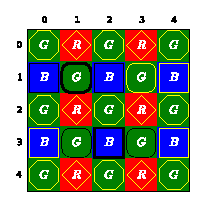
\includegraphics[width=0.27\linewidth]{fig/I^CFA_0}
	}
	\quad
	\subfigure[$I^{CFA}_x$\label{sfig:I^CFA_x}]{
		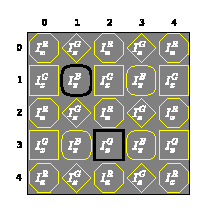
\includegraphics[width=0.27\linewidth]{fig/I^CFA_x} 
	}
	\quad
	\subfigure[Computation of $\dot{I}^l_x$\label{sfig:dotI^l_x}]{
		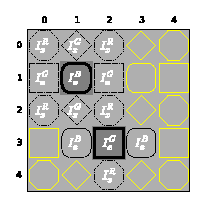
\includegraphics[width=0.27\linewidth]{fig/dotI^l_x} 
	} \\
	\subfigure[Computation of $I^{CFA}_y$\label{sfig:I^CFA_1}]{
		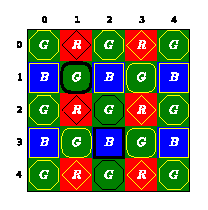
\includegraphics[width=0.27\linewidth]{fig/I^CFA_1}
	}
	\quad
	\subfigure[$I^{CFA}_y$\label{sfig:I^CFA_y}]{
		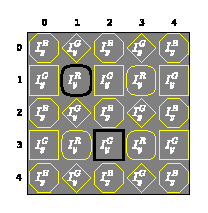
\includegraphics[width=0.27\linewidth]{fig/I^CFA_y} 
	}
	\quad
	\subfigure[Computation of $\dot{I}^l_y$\label{sfig:dotI^l_y}]{
		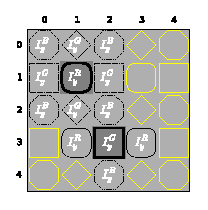
\includegraphics[width=0.27\linewidth]{fig/dotI^l_y}
	}
	\caption{First partial derivatives of a CFA image (see Eqs.~\eqref{eq:cfa_derivatives}--~\eqref{eq:I_p_y_full}), with two pixels as examples (solid bold lines). Dashed neighbours in Figs.~\subref{sfig:I^CFA_0} and~\subref{sfig:I^CFA_1} are used to compute $I^{CFA}_x$ and $I^{CFA}_y$. Dashed, dotted, and dash-and-dotted neighbours in Figs.~\subref{sfig:dotI^l_x} and~\subref{sfig:dotI^l_y} are used to compute the missing derivative components.}
	\label{fig:cfa_derivatives}
\end{figure}

\begin{figure}
	\centering
	\subfigure[$\N{x}(P)$]{
		\psfrag{P}[c][c]{$P$}
		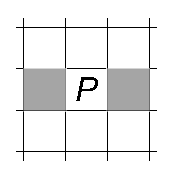
\includegraphics{fig/N^x} 
		\label{sfig:N^x}
	}
	\quad
	\subfigure[$\N{y}(P)$]{
	\psfrag{P}[c][c]{$P$}
		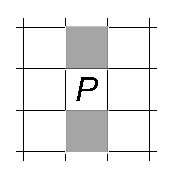
\includegraphics{fig/N^y} 
		\label{sfig:N^y}
	}
	\quad
	\subfigure[$\N{+}(P)$]{
		\psfrag{P}[c][c]{$P$}
		
\includegraphics{fig/N^+}
		\label{sfig:N^+}
	}			
	\subfigure[$\N{\times}(P)$]{
		\psfrag{P}[c][c]{$P$}
		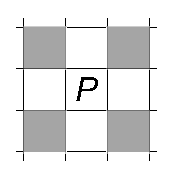
\includegraphics{fig/N^diag}
		\label{sfig:N_diag}
	}
	\caption{Neighbourhoods of a pixel $P$ used to interpolate the missing derivative components from a CFA image.}
	\label{fig:neighbourhoods}
\end{figure}

\noindent These derivatives are directly obtained from $I^{CFA}$ considered here as a simple grey scale image, and can be viewed as the result of a spatial multiplexing of the components of the same derivatives of the reference image $\mathbf{I}$ spectrally sub-sampled according to the CFA mosaic.
Because the two horizontal (or vertical) neighbours of each pixel $P$ belong to the same CFA subset $S^k$, their level difference matches with the horizontal (or vertical) derivative $I^k_x$ (or $I^k_y$) of the colour component $k$ (see Fig.~\ref{fig:cfa_derivatives}). For instance, the horizontal neighbours of the pixel $P(2,3) \in S^B$ in Fig. \ref{sfig:I^CFA_0} belong to $S^G$ and their level difference equals $2 \cdot I^G_x$ as shown in Fig. \ref{sfig:I^CFA_x}. Its vertical neighbours also belong to $S^G$ (see Fig. \ref{sfig:I^CFA_1}) and their level difference equals $2 \cdot I^G_y$ (see Fig. \ref{sfig:I^CFA_y}). The pixels in $S^G$ have to be considered separately according to whether they belong belong to $S^{G,R}$ or $S^{G,B}$. For instance, the horizontal (resp., vertical) neighbours of the pixel $P(1,1) \in S^{G,B}$ belong to $S^B$ (resp., $S^R$) and their level difference equals  $2 \cdot I^B_x$ (resp.,  $2 \cdot I^R_y$). More generally, $I^{CFA}_x$ (resp., $I^{CFA}_y$) matches with a component of $\mathbf{I}_x$ (resp., $\mathbf{I}_y$) at each pixel $P$ according to:
\begin{equation}
	\begin{array}{lcl}
		I^{CFA}_x(P) = \left\lbrace
		\begin{array}{cl}
			I^G_x(P)  & \text{if $P \in S^R \cup S^B$,}\\ 
			I^R_x(P)  & \text{if $P \in S^{G,R}$,} \\
			I^B_x(P)  & \text{if $P \in S^{G,B}$,}\\
		\end{array}\right.
		& \text{ and } &
		I^{CFA}_y(P) = \left\lbrace
		\begin{array}{cl}
			I^G_y(P)  & \text{if $P \in S^R \cup S^B$,}\\ 
			I^B_y(P)  & \text{if $P \in S^{G,R}$,} \\
			I^R_y(P)  & \text{if $P \in S^{G,B}$.}\\
		\end{array}\right.
	\end{array}
\label{eq:cfa_derivatives}
\end{equation}





%\subsubsection{CFA Deriche partial derivative}
%The previous section explains the principle of the method of Deriche and how it is applied to color images for compute the first partial derivative. In this section, we proposed to apply directly the Deriche approach on CFA images. In \ref{subsec:problem_formulation}, we saw that the CFA image can be divided into four subsets, $S^{G,R}$, $S^R$, $S^B$ and $S^{G,B}$ (see Figs.~\ref{fig: Bayer CFA and the component image}). These four subsets form four fully sub-images  (see Figs.~\ref{fig: deriche_CFA})
%
%
%
%\begin{figure}
%	\centering
%	
%	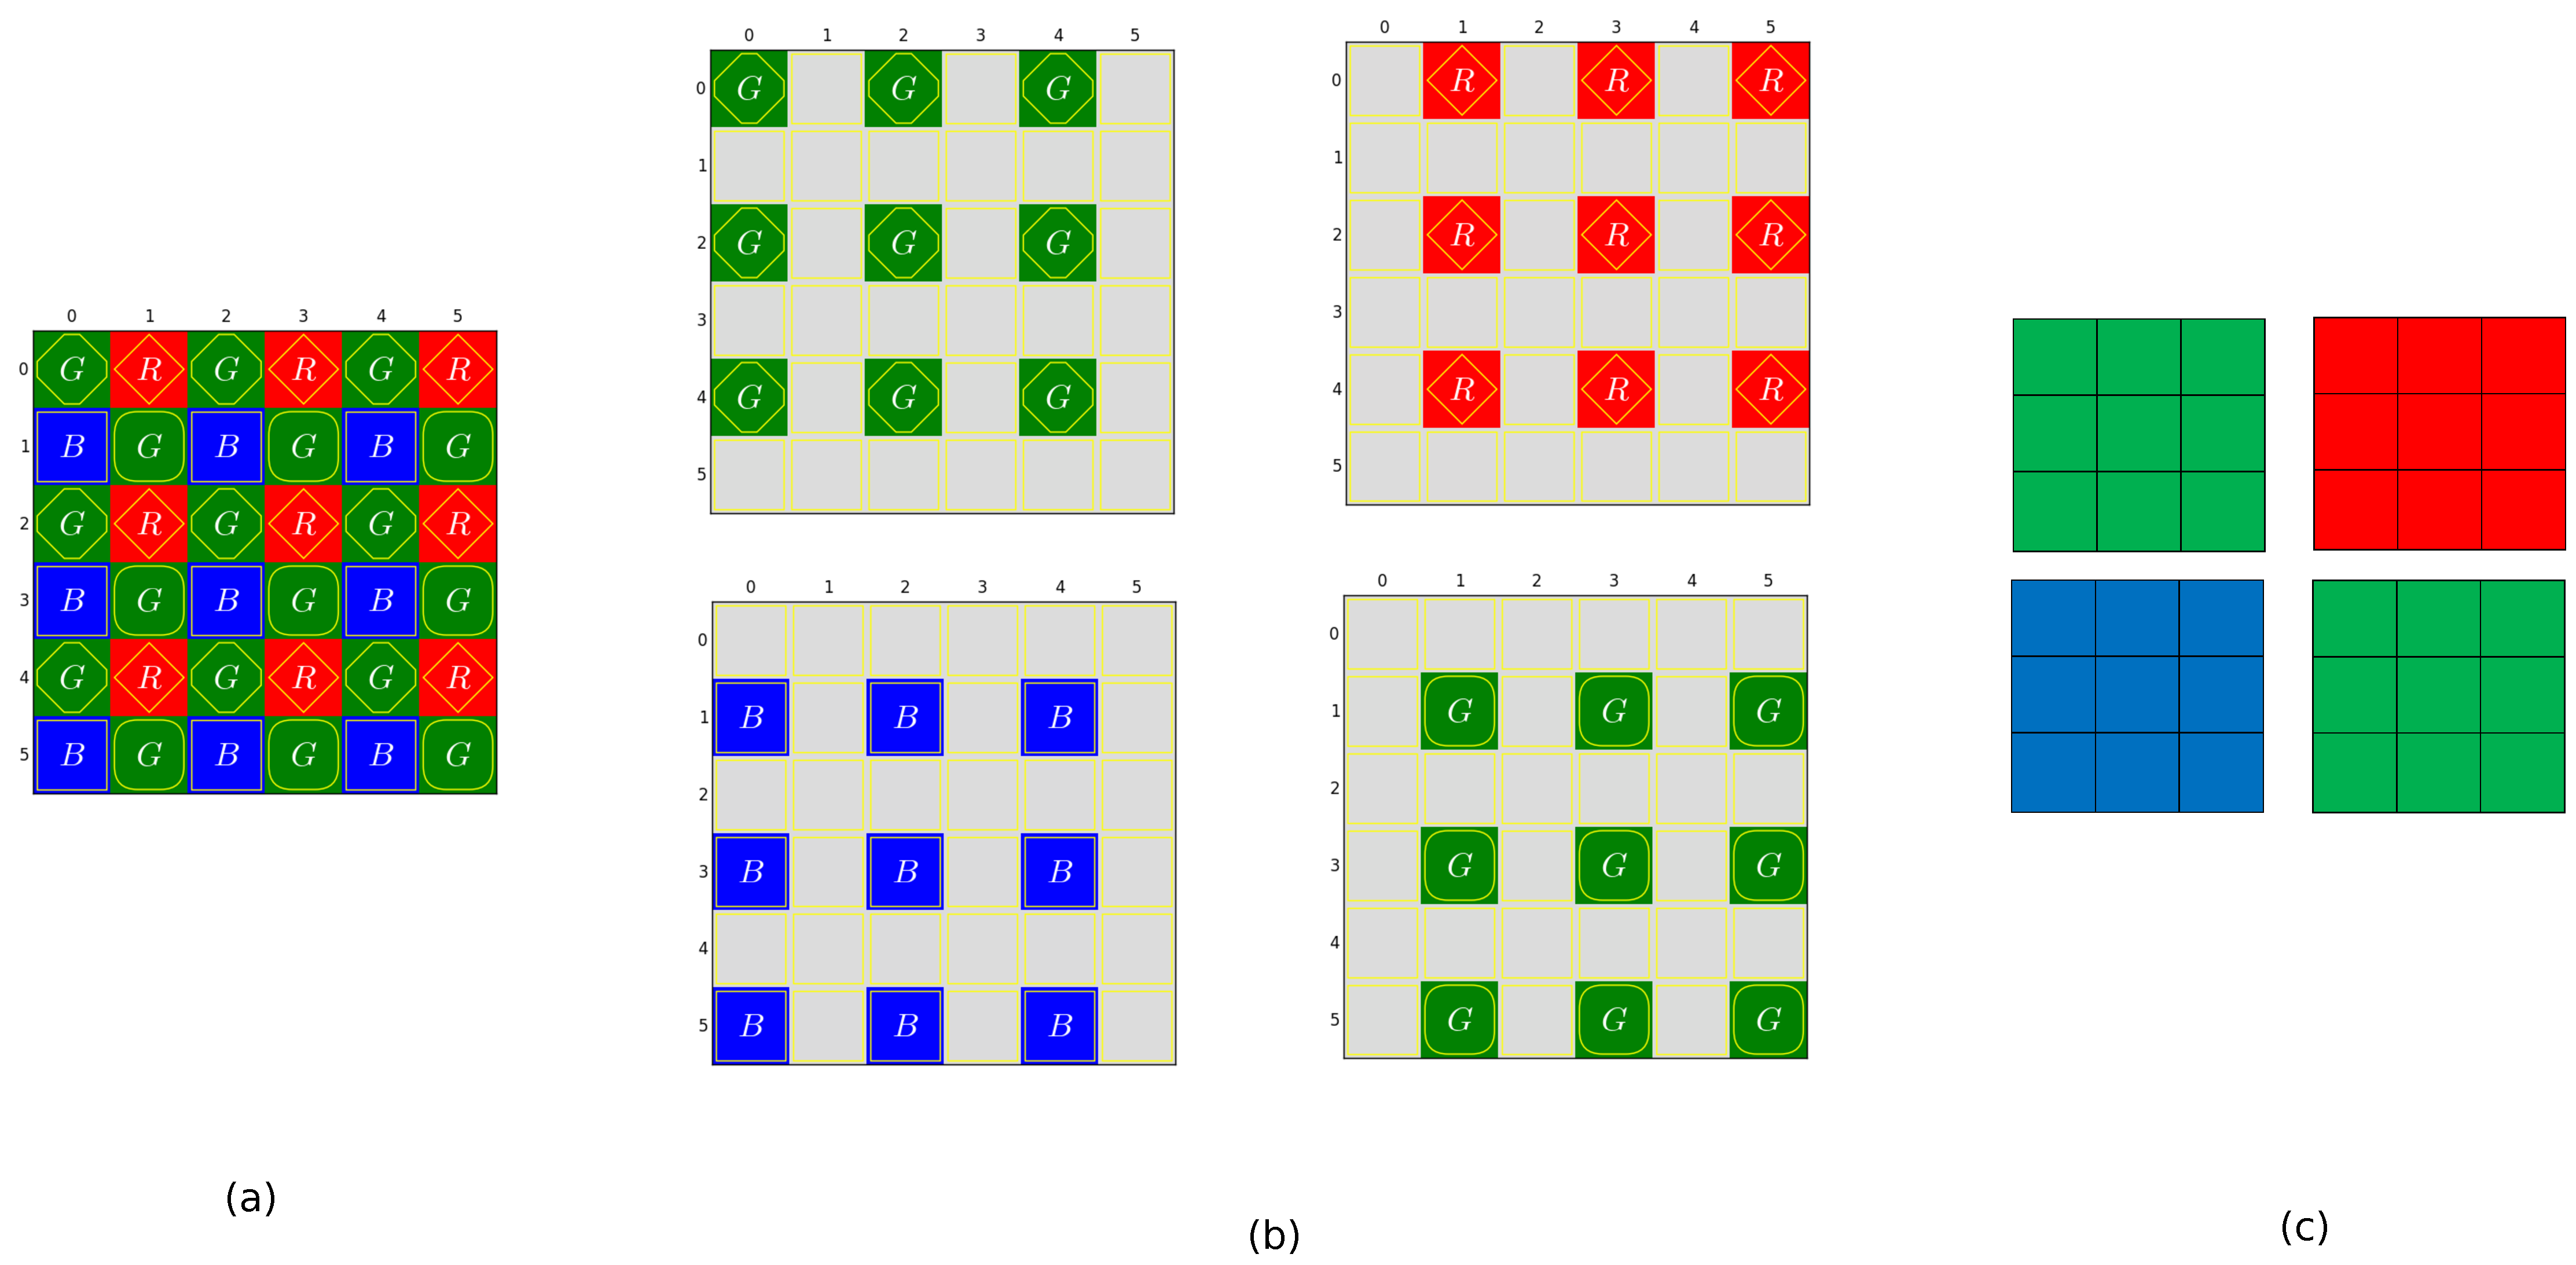
\includegraphics[width=0.9\linewidth]{fig/deriche_CFA} 		
%	
%	\caption{reorganization process of the CFA image to the application of Deriche filter (figure à refaire): (a) CFA image, (b): component-wise pixel subsets, (c):fully sub-images.}
%	\label{fig: deriche_CFA}
%\end{figure}
%
%

\subsubsection{CFA Deriche partial derivative}
In section \ref{Estimation partial derivative}.\ref{Deriche partial derivative}, to estimate the Deriche partial derivative of a colour image $\textbf{I}$, we calculated these partial derivatives in each colour component $I^k$, $k\in\{R,G,B\}$.   
Similarly, in the CFA images, the estimation of the first partial derivatives should be at the same colour component. Each colour component in the CFA image is not available at each pixel $P(x,y)$, according to figures \ref{fig:S^R}, \ref{fig:S^B} and \ref{fig:S^G}, 
the nearest neighbour of the pixel $P(x,y)\in S^k$, $k\in\{R,G,B\}$, that also belongs to $S^k$, is located at a spatial distance $d=2$ according to horizontal and vertical direction. So, to estimate the Deriche partial derivative of a CFA image at each pixel $P(x,y)$, we proceed in the same way as in section \ref{Estimation partial derivative}.\ref{Deriche partial derivative} by setting $d$ to 2. For example, the partial derivative $\D_x$  by the Deriche filter is $\D_x(x,y)=\Dmoins_x(x,y) + \Dplus_x(x,y)$ where $\Dmoins_x(x,y)$ and $\Dplus_x(x,y)$ are calculated in the same way as equations \eqref{left to right}  and \eqref{right to left} but with $d=2$.

%First, the CFA image $I^{CFA}$ is smoothed according $x$ from right to left (see equation \eqref{right to left CFA}) and from left to right (see equation \eqref{left to right CFA}): 
%
%\begin{itemize}
%	
%	\item Smoothing according $x$
%	
%	\begin{equation}
%	\label{right to left CFA}
%	\Smo {I}^{CFA^+}_x(x,y)=a_1 \cdot I^{CFA}(x,y) + a_2 \cdot I^{CFA}(x-2,y) + b_1 \cdot \Smo {I}^{CFA^+}_x(x-2,y) + b_2 \cdot \Smo {I}^{CFA^+}_x(x-4,y)
%	\end{equation}
%	
%	
%	
%	\begin{equation}
%	\label{left to right CFA}
%	\Smo {I}^{CFA^-}_y(x,y)=a_3 \cdot I^{CFA}(x+2,y) + a_4 \cdot I^{CFA}(x+4,y) + b_1 \cdot \Smo {I}^{kCFA^-}_x(x+2,y) + b_2 \cdot \Smo {I}^{CFA^-}_x(x+4,y)
%	\end{equation}
%	
%	The horizontally smoothed image $\Smo {I}^{CFA}_x$  by the Deriche filter is given by:	
%		
%	\begin{equation}
%	\Smo {I}^{CFA}_x(x,y)=\Smo {I}^{CFA^+}_x(x,y) + \Smo {I}^{CFA^-}_x(x,y)
%	\end{equation}
%	
%	
%	
%\begin{equation*}
%\begin{array}{lcl}
%Where \left\lbrace
%\begin{array}{cl}
%a_1 = m\\ 
%a_2 = m \cdot (\alpha -1)\cdot \e ^{-\alpha} \\
%a_3 = m \cdot (\alpha +1)\cdot \e ^{-\alpha}\\
%a_4 =-m \cdot \e ^{-2 \cdot \alpha}\\
%\end{array}\right.
%& \text{ and } &
%\left\lbrace
%\begin{array}{cl}
%b_1 = 2\cdot \e ^{-\alpha}\\ 
%b_2 = -\e ^{-2 \cdot \alpha} \\
%m=\frac{(1-\e^{-\alpha})^2}{1+2 \cdot \alpha \cdot \e^{-\alpha}- \e ^{-2\cdot \alpha}}\\
%\end{array}\right.
%\end{array}
%\end{equation*}
%	
%	
%\end{itemize}
%
%
%Now, for compute partial derivative according $y$, $\Smo {I}^{CFA}_x$ is passed in the vertical direction from top to bottom (see equation \eqref{ top to bottom CFA})  and bottom-up (see equation \eqref{bottom-up CFA}):
%
%
%\begin{itemize}
%	
%	
%	\item Derivative according $y$ 
%	
%	
%	\begin{equation}
%	\label{bottom-up CFA}
%	\Dplus_y(x,y) = a_5 \cdot \Smo {I}^{CFA}_x(x,y) + a_6 \cdot \Smo {I}^{CFA}_x(x,y-2) + b_1 \cdot \Dplus_y(x,y-2) + b_2 \cdot  \Dplus_y(x,y-4)
%	\end{equation}
%	
%	
%	
%	\begin{equation}
%	\label{ top to bottom CFA}
%	\Dmoins_y(x,y)= a_7 \cdot \Smo {I}^{CFA}_x(x,y+2) + a_8 \cdot \Smo {I}^{CFA}_x(x,y+4) +b_1 \cdot \Dmoins_y(x,y+2) + b_2 \cdot \Dmoins_y(x,y+4)
%	\end{equation}
%	
%	
%	The partial derivative according $y$ by the Deriche filter is given by:	
%	
%	\begin{equation}
%	\D_y(x,y)=\Dplus_y(x,y) + \Dmoins_y(x,y)
%	\end{equation}
%	
%	\begin{equation*}
%	\begin{array}{lcl}
%	Where \left\lbrace
%	\begin{array}{cl}
%	a_5 = 0\\ 
%	a_6 = 1 \\
%	a_7 = -1\\
%	a_8 = 0\\
%	\end{array}\right.
%	& \text{ and } &
%	\left\lbrace
%	\begin{array}{cl}
%	b_1 = 2\cdot \e ^{-\alpha}\\ 
%	b_2 = -\e ^{-2 \cdot \alpha} \\
%	m=\frac{(1-\e^{-\alpha})^2}{1+2 \cdot \alpha \cdot \e^{-\alpha}- \e ^{-2\cdot \alpha}}\\
%	\end{array}\right.
%	\end{array}
%	\end{equation*}
%	
%	
%\end{itemize}
%In the same way, the Deriche partial derivatives are calculated according to $x$ but $I^{CFA}$ is smoothed before according $y$.

%Therefore, if a pixel $P$ belong to $S^k$, with $k\in\{R,G,B\}$, The partial derivative according to $x$ (or according $y$) in this pixel is $I^k_x$ (or $I^k_y$).

More generally, $\D_x$ ( resp., $\D_y$) matches with a component of $\textbf{I}_x$ (resp., $\textbf{I}_y)$ at each pixel $P$ according to:

\begin{equation}
\begin{array}{lclcl}
I^k_x(P) = \D_x(P)  & \text{if $P \in S^{k}$,} & \text{ and } & I^k_y(P) = \D_y(P) & \text{if $P \in S^{k}$,}
\end{array}
\label{eq:cfa_derivatives_deriche}
\end{equation}

With $k \in \{R,G,B\}$.





\subsubsection{Fully defined partial derivative}
To get the fully-defined partial derivatives $\dot{\textbf{I}}_x$ and $\dot{\textbf{I}}_y$ of the colour image $\mathbf{I}$ from $I^{CFA}$, we need to estimate the two derivative components missing at each pixel $P$ in $I^{CFA}_x$ and $I^{CFA}_y$.
\begin{itemize}
	\item Simple partial derivative

		
		Denoting these missing components as $\dot{I}_x^l(P)$ and $\dot{I}_y^l(P)$, $l \neq k$ when $P \in S^k$, we can write:
		%$(\point {I}_x^R(P)$, $\point {I}_x^G(P)$ and $\point {I}_x^B(P))$ according $x$ and $(\point {I}_y^R(P)$, $\point {I}_y^G(P)$ and $\point {I}_y^B(P))$ according $y$, at each pixel by interpolation of available partial derivatives. To determine the partial derivatives $I^k_x$ (or $I^k_y$) of each pixel $P$ where $k \in \{R,G,B\}$, the interpolation process  retains the partial derivative available at the same location in $I_x^{CFA}$ (or $I_y^{CFA}$), and estimates the other two partial derivatives missing:
		\begin{equation}
			\dot{\textbf{I}}_x(P) = \left\lbrace
			\begin{array}{cl}
				\left( \dot{I}^R_x(P), I^{CFA}_x(P), \dot{I}^B_x(P) \right)^T & \text{if $P \in S^R \cup S^B$,}\\
				\left( I^{CFA}_x(P), \dot{I}^G_x(P), \dot{I}^B_x(P) \right)^T & \text{if $P \in S^{G,R}$,}\\
				\left( \dot{I}^R_x(P), \dot{I}^G_x(P), I^{CFA}_x(P) \right)^T & \text{if $P \in S^{G,B}$,}
			\end{array}\right.
			\label{eq:I_p_x}
		\end{equation}
		
		\noindent and $\dot{\textbf{I}}_y$ in the same way. We compute a missing derivative component $\dot{I}_{x}^l$ (or $\dot{I}_{y}^l$) at each pixel $P$ by interpolation of the derivative values $I_{x}^l$ (or $I_{y}^l$) of the same component available in a neighbourhood of $P$. This neighbourhood depends on the CFA pixel subset $S^k$ to which $P$ belongs. The four neighbourhood configurations used for this interpolation are defined in Fig. \ref{fig:neighbourhoods}, and the partial derivatives then write as:
		\begin{equation}
			\dot{\textbf{I}}_x(P) = \left\lbrace
			\begin{array}{cl}
				\left( \frac{1}{2}\cdot\sum_{Q \in \N{x}(P)} I^R_x(Q),~I^{CFA}_x(P),~\frac{1}{2}\cdot\sum_{Q \in \N{y}(P)} I^B_x(Q) \right)^T & \text{if $P \in S^R$,} \\
				\left( I^{CFA}_x(P),~\frac{1}{4}\cdot\sum_{P \in \N{+}(P)} I^G_x(P),~\frac{1}{4}\cdot\sum_{P \in \N{\times}(P)} I^B_x(P) \right)^T & \text{if $P \in S^{G,R}$,}\\
				\left( \frac{1}{4}\cdot\sum_{Q \in \N{\times}(P)} I^R_x(Q),~\frac{1}{4}\cdot\sum_{Q \in \N{+}(P)} I^G_x(Q),~I^{CFA}_x(P) \right)^T & \text{if $P \in S^{G,B}$,}\\
				\left( \frac{1}{2}\cdot\sum_{Q \in \N{y}(P)} I^R_x(Q),~I^{CFA}_x(P),~\frac{1}{2}\cdot\sum_{Q \in \N{x}(P)} I^B_x(Q) \right)^T & \text{if $P \in S^B$,}
			\end{array}\right.
			\label{eq:I_p_x_full}
		\end{equation}
		
		\noindent and:
		\begin{equation}
			\dot{\textbf{I}}_y(P) = \left\lbrace
			\begin{array}{cl}
				\left( \frac{1}{2}\cdot\sum_{Q \in \N{y}(P)} I^R_y(Q),~I^{CFA}_y(P),~\frac{1}{2}\cdot\sum_{Q \in \N{x}(P)} I^B_y(Q) \right)^T & \text{if $P \in S^R$,} \\
				\left( \frac{1}{4}\cdot\sum_{Q \in \N{\times}(P)} I^R_y(Q),~\frac{1}{4}\cdot\sum_{Q \in \N{+}(P)} I^G_y(Q),~I^{CFA}_y(P) \right)^T & \text{if $P \in S^{G,R}$,}\\
				\left( I^{CFA}_y(P),~\frac{1}{4}\cdot\sum_{Q \in \N{+}(P)} I^G_y(Q),~\frac{1}{4}\cdot\sum_{Q \in \N{\times}(P)} I^B_y(Q) \right)^T & \text{if $P \in S^{G,B}$,}\\
				\left( \frac{1}{2}\cdot\sum_{Q \in \N{x}(P)} I^R_y(Q),~I^{CFA}_y(P),~\frac{1}{2}\cdot\sum_{Q \in \N{y}(P)} I^B_y(Q) \right)^T & \text{if $P \in S^B$.}
			\end{array}\right.
			\label{eq:I_p_y_full}
		\end{equation}
		
		\noindent For instance (see Fig.~\ref{sfig:dotI^l_x}), the four diagonal neighbours of $P(1,1) \in S^{G,B}$ are used to compute $\dot{I}^R_x(P)$ while its four closest neighbours are used to compute $\dot{I}^G_x(P)$. The $x$-derivative components missing at $P(2,3) \in S^B$  are interpolated from two of its closest neighbours (i.e., vertical neighbours for $\dot{I}^R_x(P)$ and horizontal ones for $\dot{I}^B_x(P)$).
		

	\item Deriche partial derivative
	
	
		As for the simple partial derivative, we need to estimate the two derivative components missing at each pixel $P$ in $\D_x$ and $\D_y$: 	
		
	
			\begin{equation}
				\dot{\textbf{I}}_x(P) = \left\lbrace
				\begin{array}{cl}
					\left( \D_x(P), \dot{I}^G_x(P), \dot{I}^B_x(P) \right)^T & \text{if $P \in S^{R}$,}\\
					\left( \dot{I}^R_x(P), \D_x(P), \dot{I}^B_x(P) \right)^T & \text{if $P \in S^G$,}\\
					\left( \dot{I}^R_x(P), \dot{I}^G_x(P), \D_x(P) \right)^T & \text{if $P \in S^{B}$,}
				\end{array}\right.
				\label{eq:I^D_p_x}
			\end{equation}
			
			
	
		\noindent and $\dot{\textbf{I}}_y$ in the same way. The missing derivative component $\dot{I}_{x}^l$ (or $\dot{I}_{y}^l$) with ($l \neq k$) at each pixel $P$ is given by:	
	
	
	
\end{itemize}	
	
%	
%		\noindent and $\dot{\textbf{I}}_y$ in the same way. We compute a missing derivative component $\dot{I}_{x}^l$ (or $\dot{I}_{y}^l$) at each pixel $P$ by interpolation of the derivative values $I_{x}^l$ (or $I_{y}^l$) of the same component available in a neighbourhood of $P$. This neighbourhood depends on the CFA pixel subset $S^k$ to which $P$ belongs. The partial derivatives then is written as:
		
%	
%		\begin{equation}
%		\dot{\textbf{I}}_x(P) = \left\lbrace
%		\begin{array}{cl}
%			\left( \D_x(P), ~\frac{1}{2} max \left(|\sum_{Q \in \N{x}(P)} I^G_x(Q)|, |\sum_{Q \in \N{y}(P)} I^G_x(Q)|\right),~\frac{1}{4}\cdot\sum_{Q \in \N{\times}(P)} I^B_x(Q) \right)^T & \text{if $P \in S^R$} \\
%			\left( \frac{1}{2}\cdot\sum_{Q \in \N{x}(P)} I^R_x(Q),~\D_x(P),~\frac{1}{2}\cdot\sum_{Q \in \N{y}(P)} I^B_x(Q) \right)^T & \text{if $P \in S^{G,R}$,}\\
%			\left( \frac{1}{2}\cdot\sum_{Q \in \N{y}(P)} I^R_x(Q),~\D_x(P),~\frac{1}{2}\cdot\sum_{Q \in \N{x}(P)} I^B_x(Q) \right)^T & \text{if $P \in S^{G,B}$,}\\
%			\left( \frac{1}{4}\cdot\sum_{Q \in \N{\times}(P)} I^R_x(Q), ~\frac{1}{2} max \left(|\sum_{Q \in \N{x}(P)} I^G_x(Q)|, |\sum_{Q \in \N{y}(P)} I^G_x(Q)|\right),~\D_x(P) \right)^T & \text{if $P \in S^B$,}
%		\end{array}\right.
%		\label{eq:I^D1_p_x_full}
%		\end{equation}
		




		If $\left(|\frac{1}{2}\cdot\sum_{Q \in \N{x}(P)} I^G_x(Q)|>|\frac{1}{2}\cdot\sum_{Q \in \N{y}(P)} I^G_x(Q)|\right)$ in the case where $P \in (S^R \cup S^B)$ :
		
		\begin{equation}
		\dot{\textbf{I}}_x(P) = \left\lbrace
		\begin{array}{cl}
		\left( \D_x(P), ~\frac{1}{2}\cdot\sum_{Q \in \N{x}(P)} I^G_x(Q),~\frac{1}{4}\cdot\sum_{Q \in \N{\times}(P)} I^B_x(Q) \right)^T & \text{if $P \in S^R$} \\
		\left( \frac{1}{2}\cdot\sum_{Q \in \N{x}(P)} I^R_x(Q),~\D_x(P),~\frac{1}{2}\cdot\sum_{Q \in \N{y}(P)} I^B_x(Q) \right)^T & \text{if $P \in S^{G,R}$,}\\
		\left( \frac{1}{2}\cdot\sum_{Q \in \N{y}(P)} I^R_x(Q),~\D_x(P),~\frac{1}{2}\cdot\sum_{Q \in \N{x}(P)} I^B_x(Q) \right)^T & \text{if $P \in S^{G,B}$,}\\
		\left( \frac{1}{4}\cdot\sum_{Q \in \N{\times}(P)} I^R_x(Q),~\frac{1}{2}\cdot\sum_{Q \in \N{x}(P)} I^G_x(Q),~\D_x(P) \right)^T & \text{if $P \in S^B$,}
		\end{array}\right.
		\label{eq:I^D1_p_x_full}
		\end{equation}
		
		
		If $\left(|\frac{1}{2}\cdot\sum_{Q \in \N{x}(P)} I^G_x(Q)|<|\frac{1}{2}\cdot\sum_{Q \in \N{y}(P)} I^G_x(Q)|\right)$, $\dot{I}^G_x(P)=\frac{1}{2}\cdot\sum_{Q \in \N{y}(P)} I^G_x(Q)$ where $P \in (S^R \cup S^B)$.
		
		
		

		\noindent and $\dot{\textbf{I}}_y(P)$ is calculated in the same way as $\dot{\textbf{I}}_x(P)$.  


				

		
%		\noindent For instance (see Fig.~\ref{sfig:dotI^l_x}), the four diagonal neighbours of $P(1,1) \in S^{G,B}$ are used to compute $\dot{I}^R_x(P)$ while its four closest neighbours are used to compute $\dot{I}^G_x(P)$. The $x$-derivative components missing at $P(2,3) \in S^B$  are interpolated from two of its closest neighbours (i.e., vertical neighbours for $\dot{I}^R_x(P)$ and horizontal ones for $\dot{I}^B_x(P)$).
		
	
	
	


%-----------------------------------------------------------------------
\subsection{Canny edge detection}
\label{Canny edge detection}
From the above fully-defined partial derivatives according to $x$ and $y$, Di Zenzo's approach (see Sect.~\ref{subsec:colour_gradient}) allows us to estimate the norm $||\nabla \mathbf{I}||$ and the direction $\theta^{*}$ of the vector gradient directly from CFA image.
Computing binary edge image requires two steps: the extraction of the local maxima by removing the non local maxima of $||\nabla \mathbf{I}||$ along the direction $\theta^{*}$, followed by local maxima image thresholding. We'll see more on this in part section \ref{subsec:Experimental procedure}.     


%\begin{itemize}
%	
%	\item \textbf{Non local maxima image}
%	
%		\begin{itemize}
%			\item Let $P_1(x,y)$ and $P_2(x,y)$ the pixels situated on either side of $P(x,y)$ in the direction $\theta^{*}(x,y)$ of the gradient. The pixel $P_1(x,y)$ is neighboring pixel of $P (x,y)$  located in the direction $\theta^{*}(x,y)$ and $P_2(x,y)$ is also a neighboring pixel to $P(x,y)$ but in the direction opposite.
%			\item We compare the gradient norm in $P(x,y)$ with the gradient norm in $P_1(x,y)$ and in $P_2(x,y)$:
%			
%			If $||\nabla \mathbf{I}(P)|| \geq ||\nabla \mathbf{I}(P_1)||$ and $||\nabla \mathbf{I}(P)|| \geq ||\nabla \mathbf{I}(P_2)||$ so $P(x,y)$ is a local maxima.
%			
%			\item set to $0$ the gradient norm for non-local maxima pixels.	
%		\end{itemize}
%		
%	\item \textbf{Edge image}
%\end{itemize}
%
%To obtain the edge image, thresholding is applied to the image of local maxima $I_M$. Let $Th$ the chosen threshold,  the pixel $I_M(x,y)$ is classified as a edge pixel if $I_M(x,y) > Th$ and takes the value $255$. Else $I_M(x,y)$ takes $0$ as value if $I_M(x,y)<Th$. All the pixels with $255$ as value form the edge image $I_E$. We'll see more on this in part section \ref{subsec:Comparison and results}. 


	
\section{Results}
\label{sec:Results}
This section demonstrates the relevance of using the CFA image in edge detection. This new approach of edge detection is compared with edge detection at demosaicing image.To evaluate the edge detection results, we have conducted a number of tests.   



\subsection{Experimental procedure}
\label{subsec:Experimental procedure}
 To assess the robustness of different edge detection approach against edge orientation, we build a first synthesis image that contains several hexadecagons. We choose this image because it contains 16 different orientations belonging to $[-\pi,\pi[$ with a step of $\frac{\pi}{8}$, which coincides with the possible values that can take $\theta^{*}$ (See the section \ref{subsec:colour_gradient}).
 To take a larger range of edge orientation, we build a second synthesis image that contains several concentric circles ( see fig \ref{fig:Images of circles and hexadecagon}). The two synthesis images contains $13$ concentric circles (or hexadecagons) build around a main circle (or hexadecagon). The distance between the main circle (or hexadecagon) and the first concentric circle is setting by a pixel, this distance increases by one pixel for each new concentric circle (or hexadecagon). The distance between the last concentric circles (or hexadecagon) and the penultimate circle (or hexadecagon) will be $14$ pixels. In the same way, the thickness of the first circle (or hexadecagon) is set to 1 pixel to  reach $14$ pixels for the last concentric circles (or hexadecagon).
    




\begin{figure}
	\centering
	\subfigure[hexadecagon]{
		\psfrag{P}[c][c]{$P$}
		
\includegraphics[width=0.22\linewidth]{fig/hexa.eps} 
		\label{sfg:hexadecagon}
	}
	\quad
	\subfigure[True edge]{
		\psfrag{P}[c][c]{$P$}
		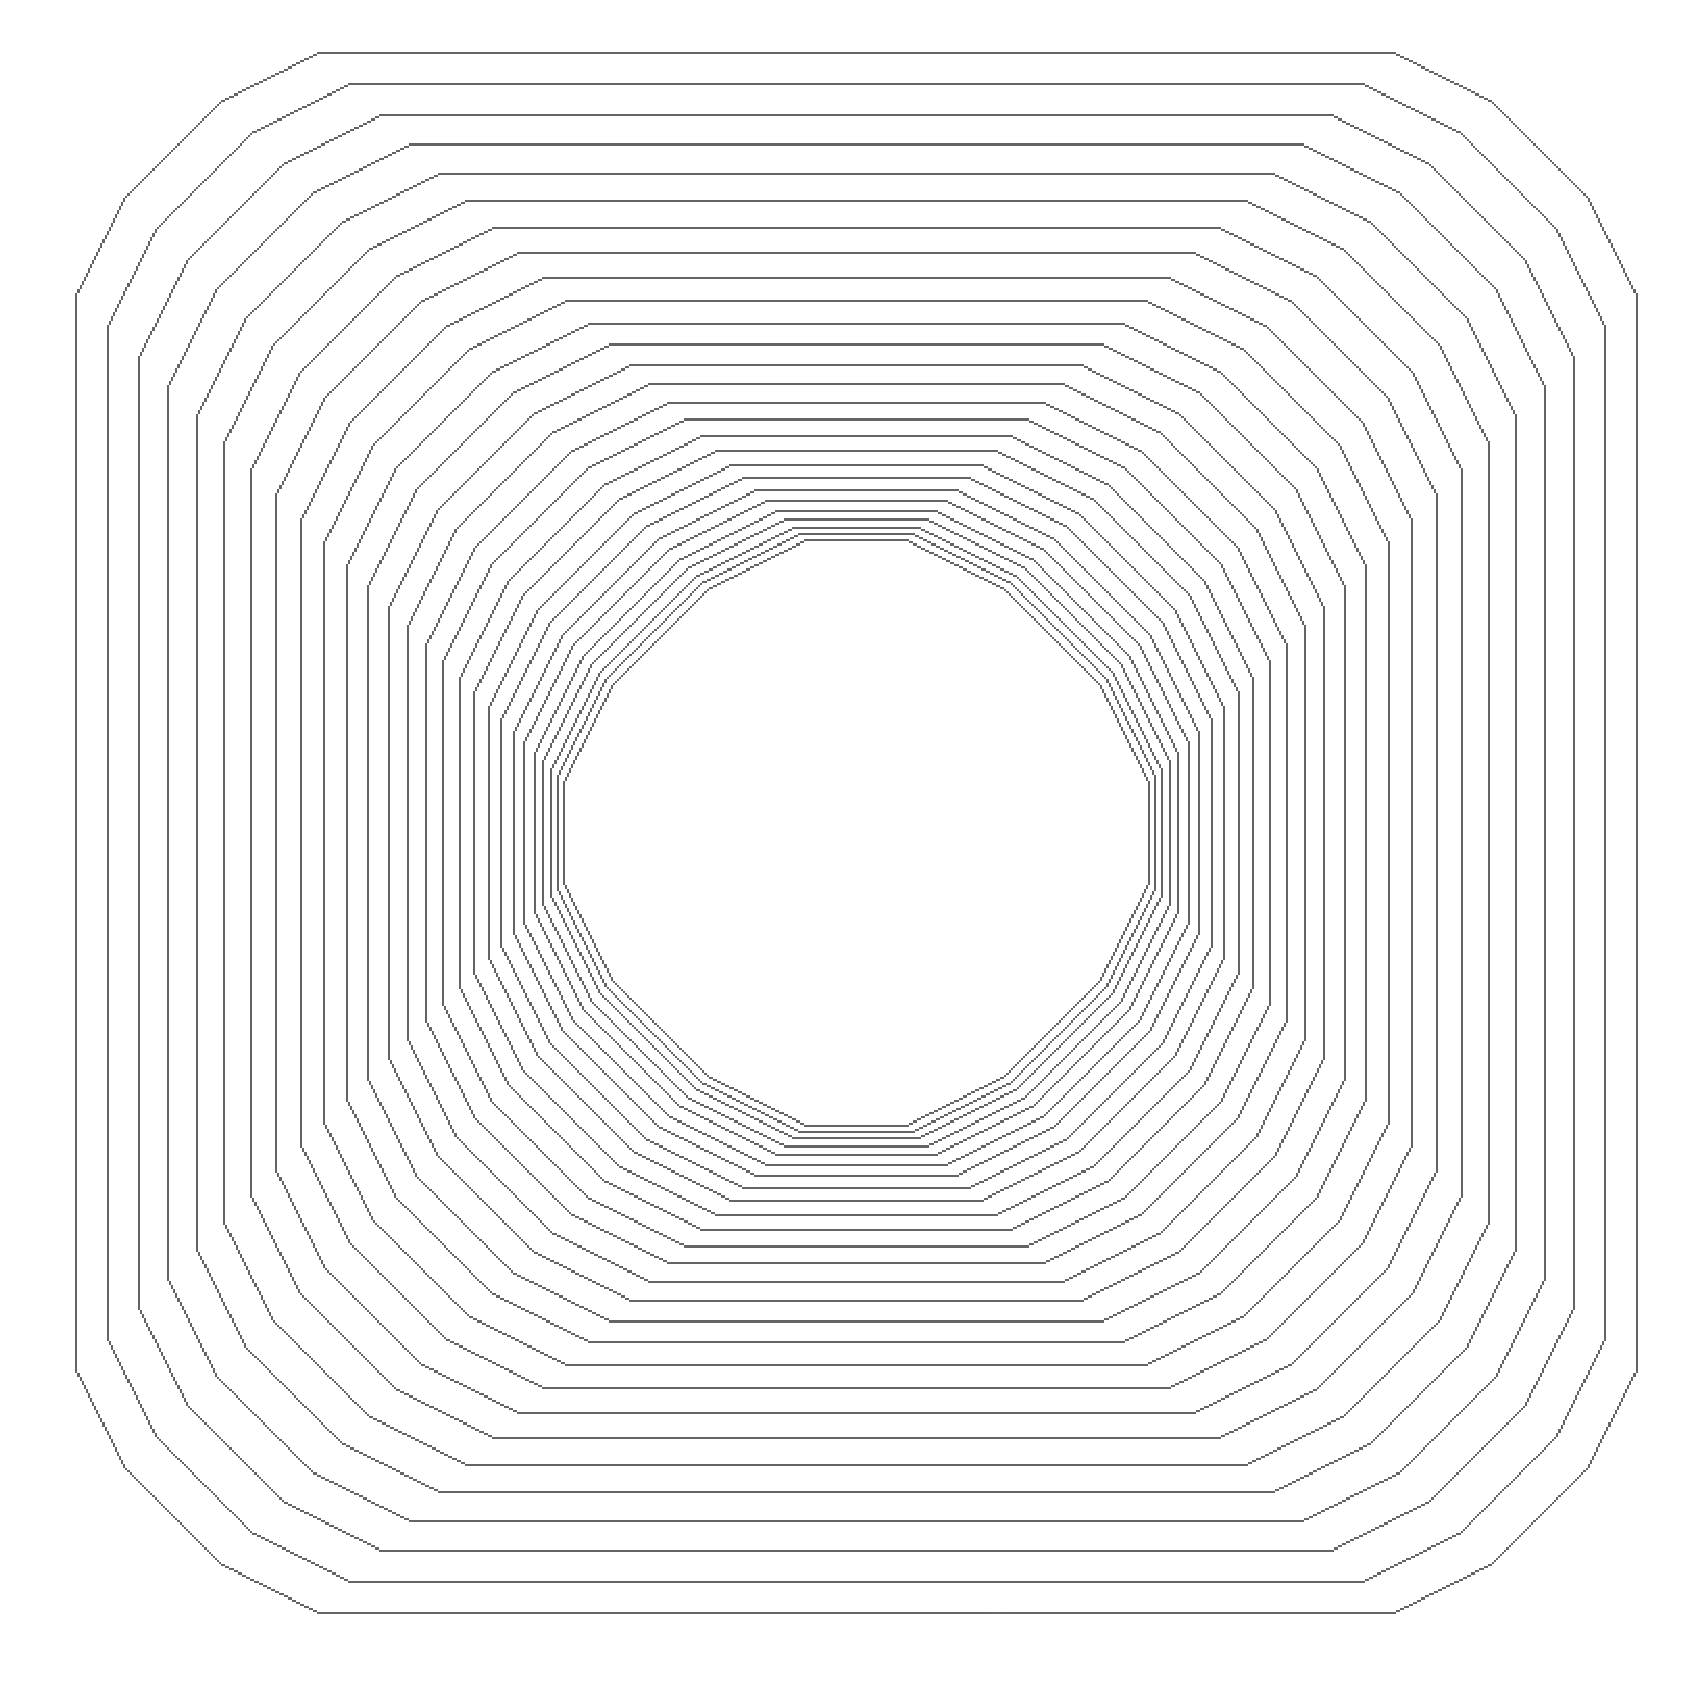
\includegraphics[width=0.22\linewidth]{fig/True_edge_hexa_inv.eps} 
		\label{sfig:True edge_hexa}
	}
	\quad
	\subfigure[circles]{
		\psfrag{P}[c][c]{$P$}
		
\includegraphics[width=0.22\linewidth]{fig/disk.eps}
		\label{sfig:circles}
	}		
	\subfigure[True edge]{
		\psfrag{P}[c][c]{$P$}
		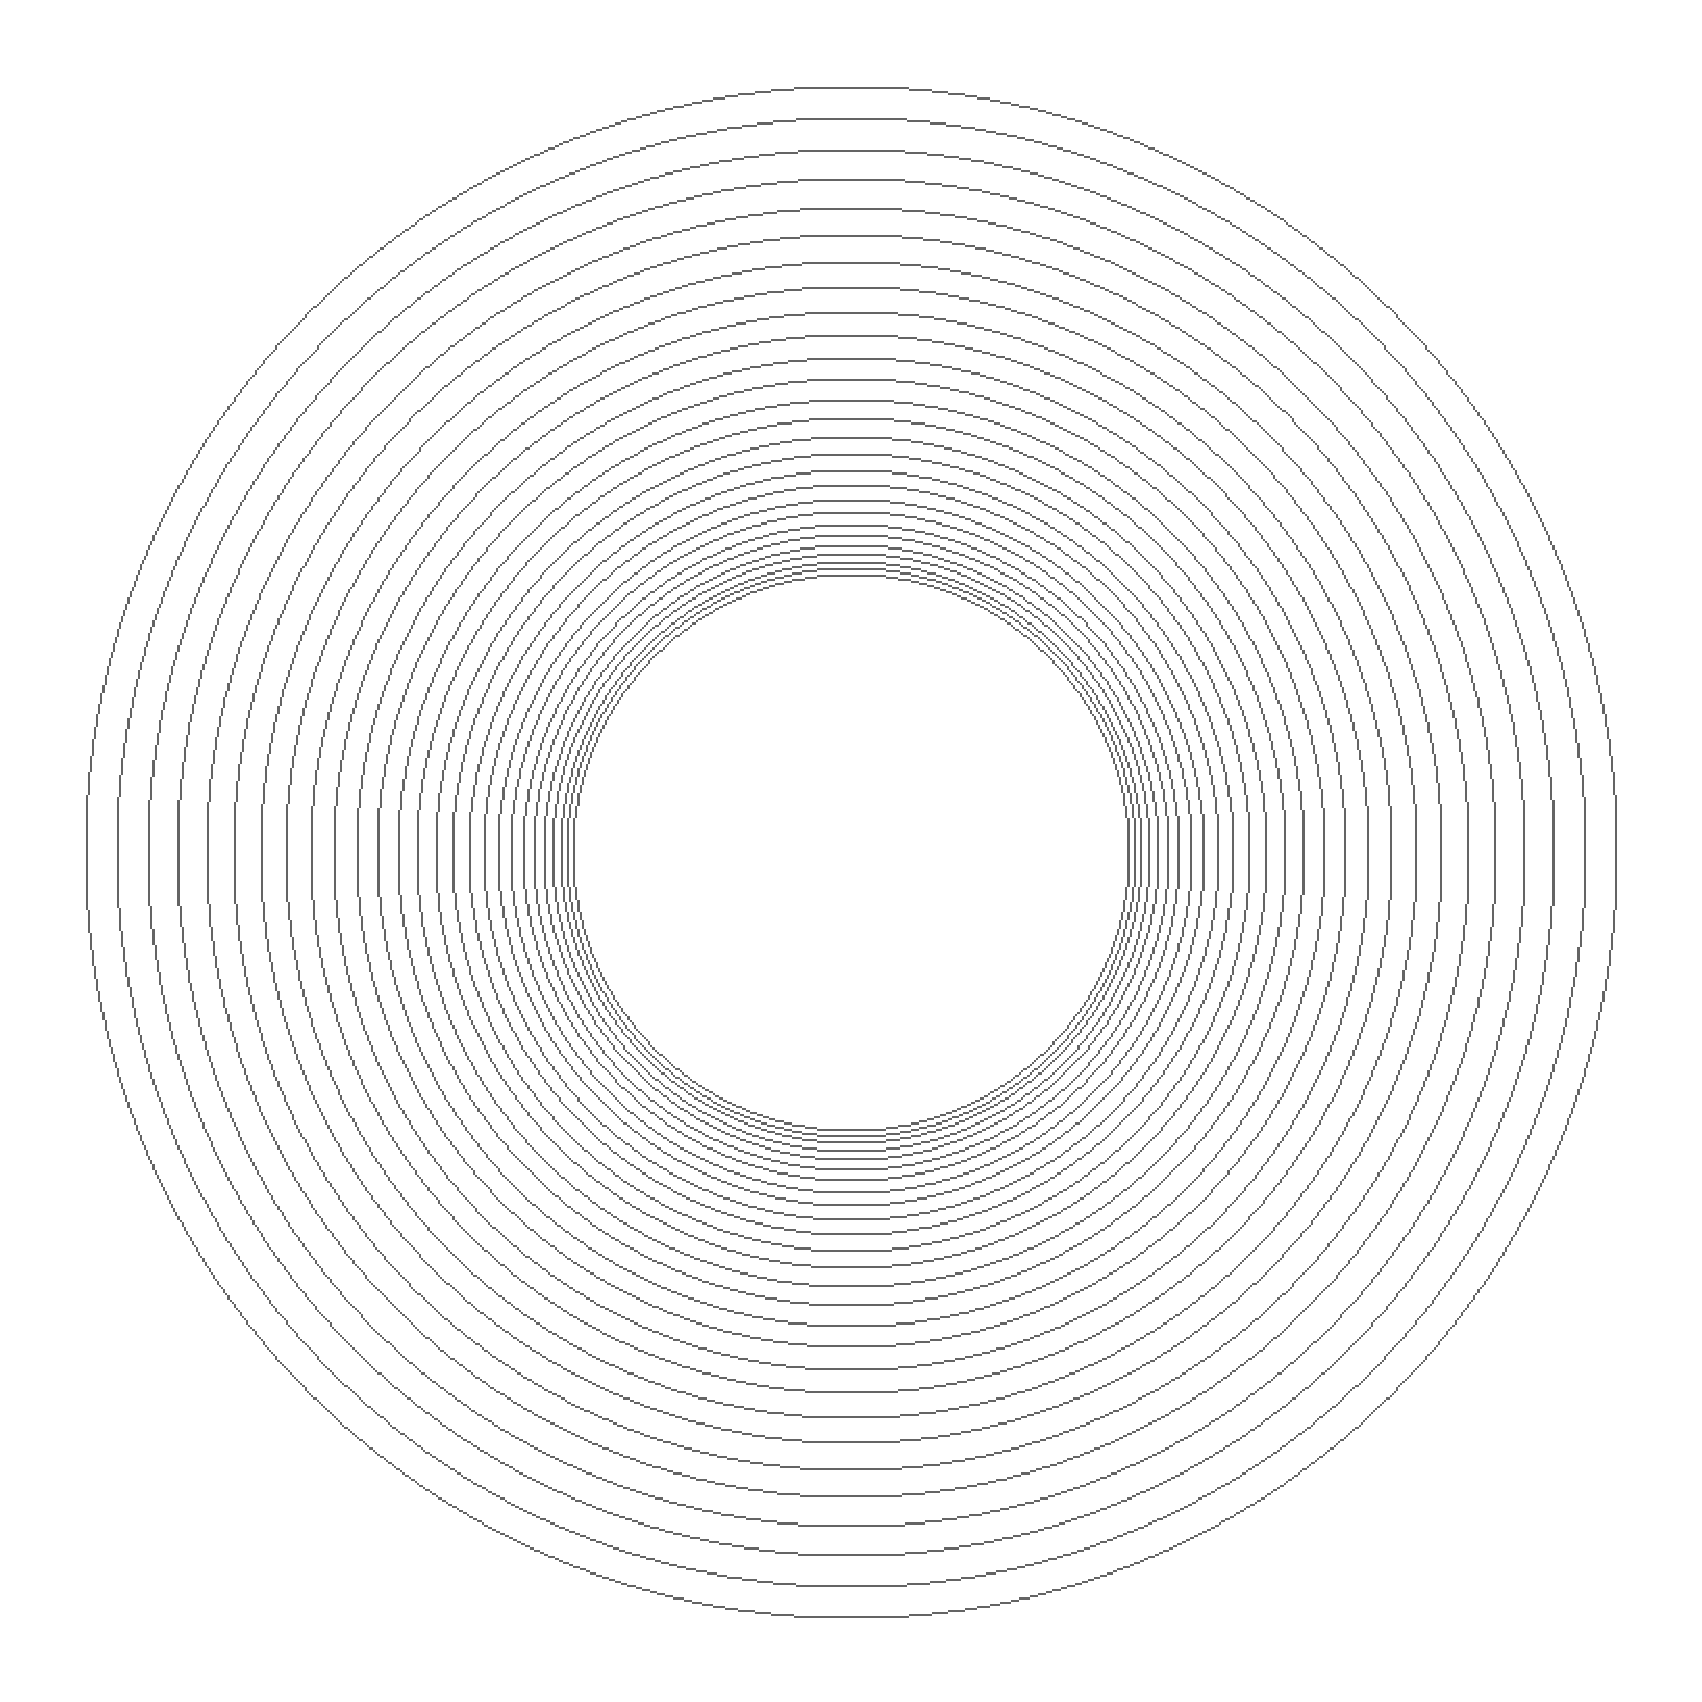
\includegraphics[width=0.22\linewidth]{fig/True_edge_circles_inv.eps} 
		\label{sfig:true_edge_circle}
	}
	\caption[Images of circles and hexadecagon.]{Images of circles and hexadecagon.}
	\label{fig:Images of circles and hexadecagon}
\end{figure}






\subsubsection{Ground truth image}
\label{sec:Ground truth image}
To build these reference images, we took into account several parameters which influence the edge detection, such as changes in colour component levels and transition width. 
The transition width depends of the standard deviation of a Gaussian Blur applied to the image (See fig \ref{fig: image_reference_transition_width}). In the horizontal (or vertical) direction the standard deviation of the Gaussian $\rho=0$ corresponds to a transition width  $tw=1$ pixel, standard deviation of the Gaussian $\rho=1$ it corresponds to $tw=3$ pixels and standard deviation of the Gaussian $\rho=2$ it corresponds to $tw=7$ pixels. 


\begin{figure}
	\centering
	\subfigure[$\rho=0$,~$tw=1$]{
		\psfrag{P}[c][c]{$P$}
		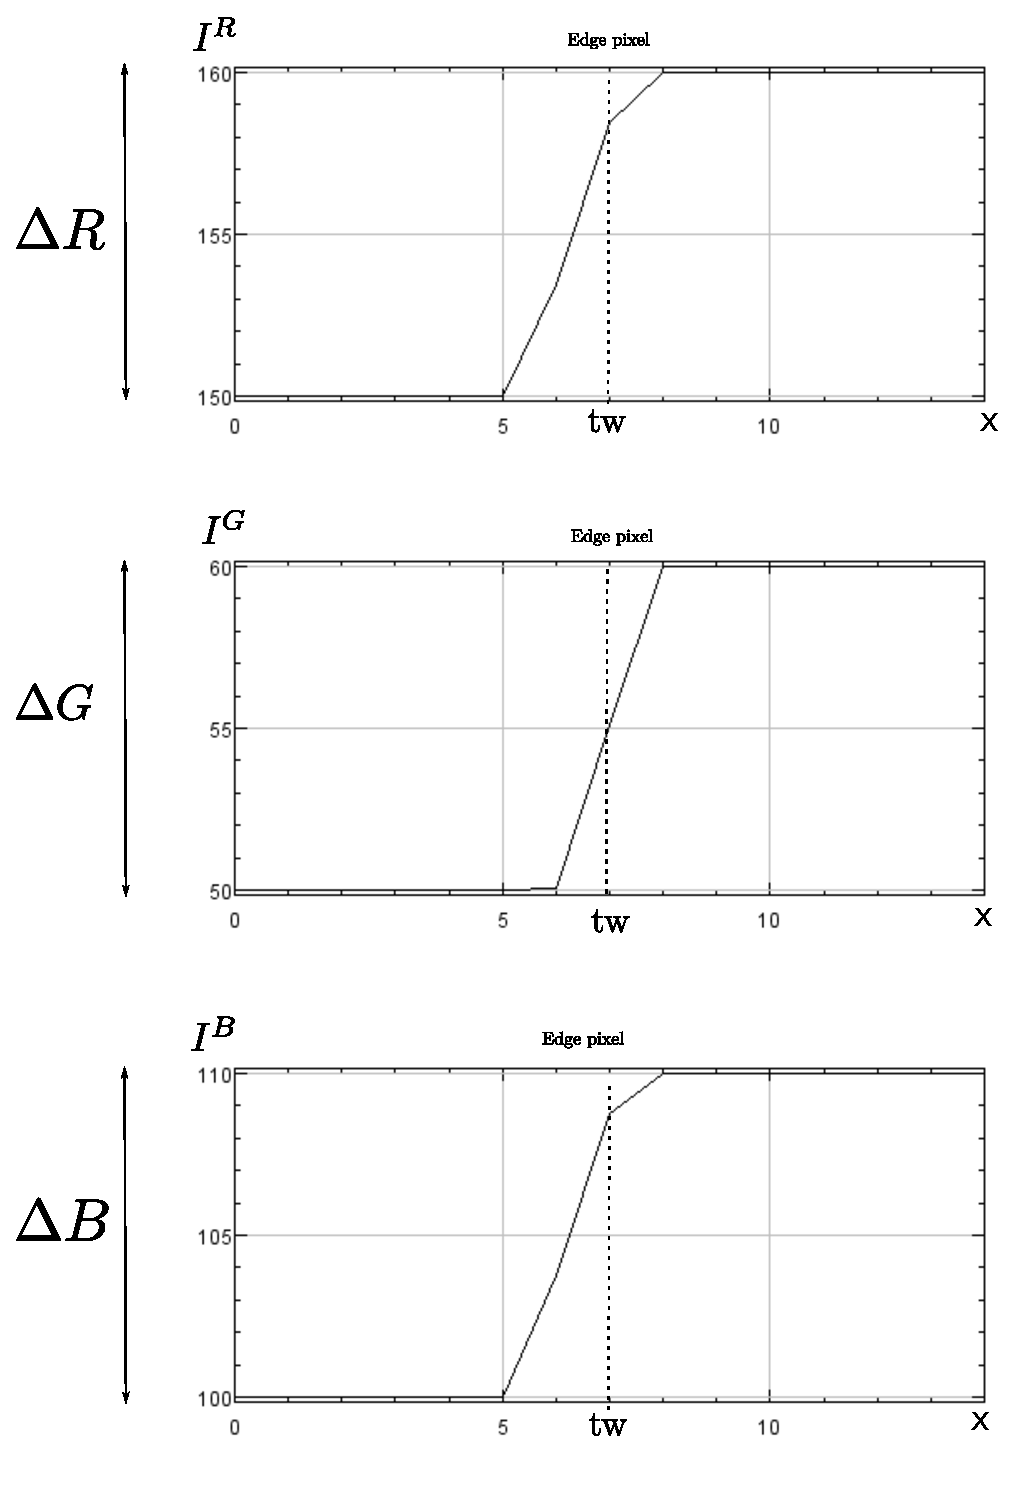
\includegraphics[width=0.48\linewidth]{fig/width_reference_image_sigma_0} 
		\label{sfig: image_reference_sigma_0}
	}
	\subfigure[$\rho=1$,~$tw=3$]{
		\psfrag{P}[c][c]{$P$}
		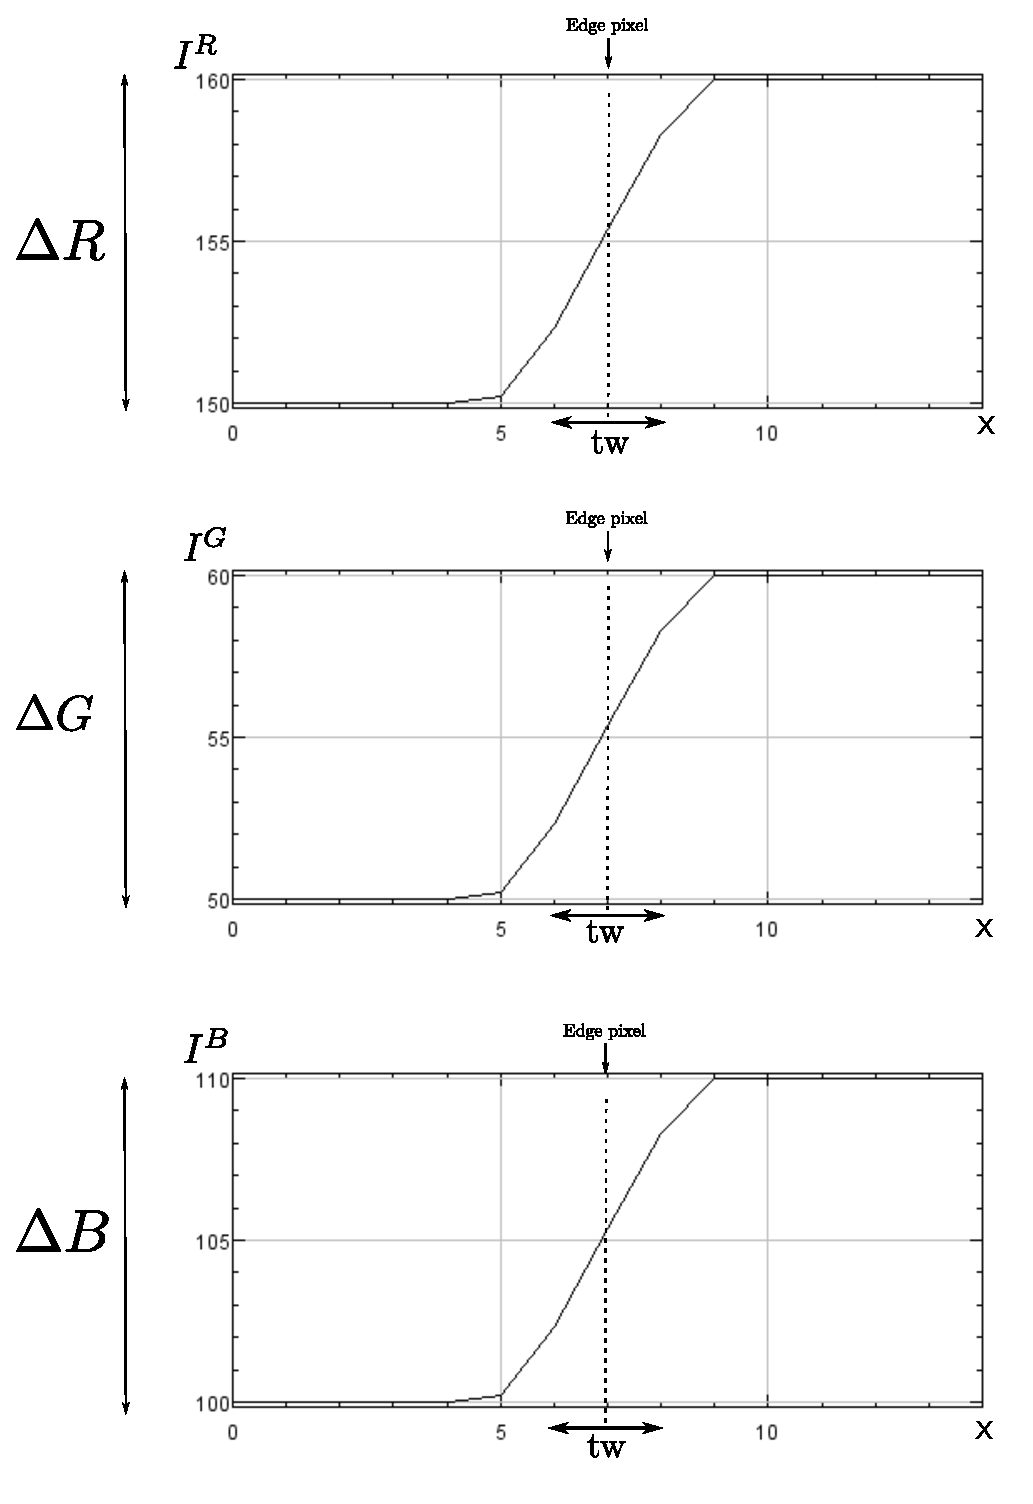
\includegraphics[width=0.48\linewidth]{fig/width_reference_image_sigma_1} 
		\label{sfig: image_reference_sigma_1}
	}
	\caption[width reference image.]{width reference image: $R=150$, $G=50$ , $B=100$, $\Delta R=\Delta G=\Delta B=10$ and noiseless.}
	\label{fig: image_reference_transition_width}
\end{figure}





%
%\begin{figure}
%	\centering
%	\subfigure[Reference image: tw=1, $\sigma _{noise}=6$, $R=150$, $G=50$ et $B=100$, $\Delta R=\Delta G=\Delta B=10$]{		
%		
\includegraphics[width=0.8\linewidth]{fig/width_reference_image_noise} 
%		\label{sfig:N^4x}
%	}
%	\quad
%	\subfigure[Reference image: tw=1, $\sigma _{noise}=6$, $R=100$, $G=150$ et $B=50$, $\Delta R=\Delta G=\Delta B=10$]{	
%		\includegraphics[width=0.8\linewidth]{fig/width_reference_image_noise_green} 
%		\label{sfig:N4^y}
%	}
%	
%	\caption{Adding Gaussian noise according to the levels of the color components  in the reference image.}
%	\label{fig:neighbourhoo4ds}
%\end{figure}

To measure the noise detection robustness, we corrupt the image by a additive Gaussian noise. Zhang et $al.$ propose to add a noise independently for each channel \cite{zhang_ip_2007}. Effectively, to add a Gaussian noise with a standard deviation $\sigma$ to a colour image $\textbf{I}$, we added separately to each image channel $I^k$ a Gaussian noise $\noise^k$ with a standard deviation $\sigma_k$ which is proportional to the energy $E^k$:    



\begin{equation}	
	\begin{array}{cl}
		\sigma_k =\sigma \cdot \left(\frac{E^k}{E}\right) & \text{with $E^k$ Energy of the channel $k$}
	\end{array}
	\label{eq:sigma_k}
\end{equation}

Where: $E=E^R + E^G + E^B$

$k\in\{R,G,B\}$,

Therefore, the noisy channel $I^k_N$ is obtained as: $I^k_N(x,y)= I^k(x,y) + \noise^k(x,y)$.



%\begin{equation}
%I^k_N(x,y)= I^k(x,y) + \eta^k(x,y)
%\end{equation}
%Where $I^k_N(x,y)$ is the notation for the channel $k$ noisy image.



%Where $\sigma_k$, $k=\{R,G,B\}$,  is the standard deviation of the Gaussian noise added for each channel $k$.
%  
%$\eta^k\sim\noise_{\sigma_k}$
%
%with $\sigma_k$



















\subsubsection{Measuring the edge detection quality}
\label{Measuring the edge detection quality}
In literature, a widely used similarity measure between ground truth contours and detected edges is Pratt's Figure of Merit (FOM) \cite{abdou_pieee_1979}:

\begin{equation}
FOM = \frac{1}{max(card(I^T),card(I^E))} \times \sum_{P\in I^E}\frac{1}{1+\frac{dis^2(P)}{9}}
\end{equation}


where: $I^T$: true edge, $I^E$: detected edge and $dis$: the distance between the pixel $P$ of $I^T$ and  the nearest pixel of $I^E$.
The edge detection is considered as good if FOM is close to $1$ and poor when this value tends to $0$.

We saw in the section \ref{Canny edge detection} that the computing of the binary edge image requires the thresholding of the local maxima image. To choose the best threshold $Th$, we thresheld the local maxima image with all possible values of $Th$. Then we compute the Pratt's Figure of Merit criterion (FOM) between ground truth contours and each image obtained with the threshold $Th$. The selected threshold corresponds to the best FOM. So, for different edge detection approach, we have the best threshold corresponding to the best FOM. From the FOM criterion, we can evaluate the edge detection quality of different edge detection approach. We detail these different approaches and the evaluation results in the next section.       





\subsection{Comparison and results}
\label{subsec:Comparison and results}
















\subsection{Discusion}
\label{subsec:Discusion}











%----------------------------------------------------------------------------------------
%	REFERENCE LIST
%----------------------------------------------------------------------------------------


\bibliographystyle{plain} % Style bibliographique auteur-date. Pour un style avec numéro, remplacer par : \bibliographystyle{plain/alpha}
\bibliography{biblio} %Pour faire sa bibliographie avec Bibtex



%------------------------------------------------









%\begin{thebibliography}{99} % Bibliography - this is intentionally simple in this template
%\bibitem[Figueredo and Wolf, 2009]{Figueredo:2009dg}
%Figueredo, A.~J. and Wolf, P. S.~A. (2009).
%\newblock Assortative pairing and life history strategy - a cross-cultural
%  study.
%\newblock {\em Human Nature}, 20:317--330.
 
%\end{thebibliography}

% %\end{multicols}{2}

\end{document}
